\documentclass{article}
\usepackage{ctex}
\usepackage[a4paper,left=10mm,right=10mm,top=15mm,bottom=15mm]{geometry}
\usepackage{graphicx}
\usepackage{amsfonts,amssymb}
\usepackage{amsmath}
\usepackage{biblatex}
\usepackage{hyperref}
\usepackage{color}
\usepackage{titlesec}
\usepackage{titletoc}

\title{VI-SLAM系统可观性和一致性分析}
\author{张谦}
\date{2020年03月06日}
\begin{document}
\maketitle
\tableofcontents
\newpage
\section{结论}
(1)对于状态估计问题,并不一定需要保证“无偏估计”,才会得到ATE较小的估计值;如果能保证系统的“一致性”,
得到更有效的估计值,尽管是“有偏的”,也可能得到ATE较小的估计状态;
\par
(2)VI-SLAM系统,不可观维度有4维:全局坐标系下的平移和绕重力方向的旋转(yaw角);
状态估计过程中的不可观维度如果和实际不可观维度不等,则会导致系统存在“一致性”问题,进而导致估计误差变大;
\par
(3)Robocentric-VIO由于采用robocentric而非world-centric的状态估计方式,能够保证系统不可观维度一直不变,
进而保证系统的“一致性”,因此可以得到较精确的估计状态。


\section{无偏估计、有效性和一致性}
现实中常常有这样的问题,比如图\ref{figs:heightGaussian},想知道全体女性的身高
均值$\mu$,但是没有办法把每个女性都进行测量,只有抽样
一些女性来估计全体女性的身高:
\begin{figure}[ht]
    \centering
    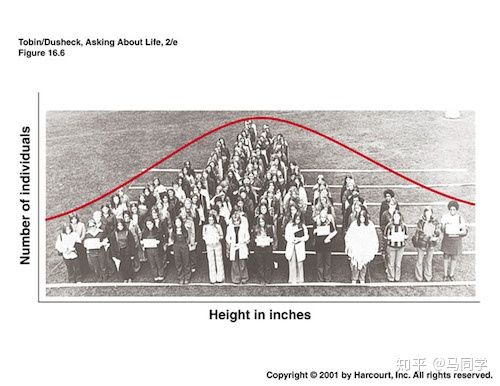
\includegraphics[width=10cm]{figure1.jpg}
    \caption{身高高斯分布示意图}
    \label{figs:heightGaussian}
\end{figure}

那么根据抽样数据怎么进行推断?什么样的推断方法才称为“好”?$\left[1\right]$
\subsection{无偏性}
比如说我们采样到的女性身高分别为:
\begin{equation}
\{x_1,x_2,\dots,x_n\}
\end{equation}
那么,
\begin{equation}
\bar{X}=\frac{x_1+x_2+\dots+x_n}{n}
\end{equation}
是对$\mu$不错的一个估计,为什么?因为它是无偏估计。\par
首先,真正的全体女性的身高均值$\mu$,我们是不知道的,只有上帝才知道,在
图2中就画为虚线,通过采样计算出$\bar{X}$会发现,不同采样得到的$\bar{X}$是
围绕$\mu$左右波动的。这有点像打靶,如图3,只要命中在靶心周围,还算不错的成绩,这就是无偏的。

\begin{figure}[ht]
    \centering
    \begin{minipage}[t]{4.5cm}
        \centering
        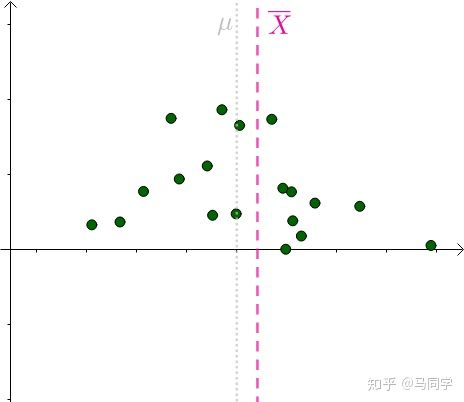
\includegraphics[width=4.5cm]{figure2.jpg}
        \caption{采样计算$\bar{X}$}
        \label{figs:SmapleExample}
    \end{minipage}
    \hspace{1cm}
    \begin{minipage}[t]{4cm}
        \centering
        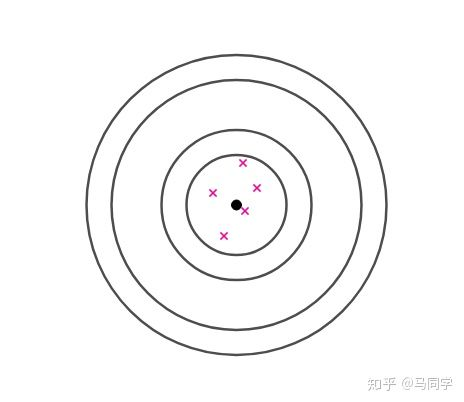
\includegraphics[width=4cm]{figure3.jpg}
        \caption{打靶例子}
        \label{figs:ShotExample1}
    \end{minipage}
    \hspace{1cm}
    \begin{minipage}[t]{6.7cm}
        \centering
        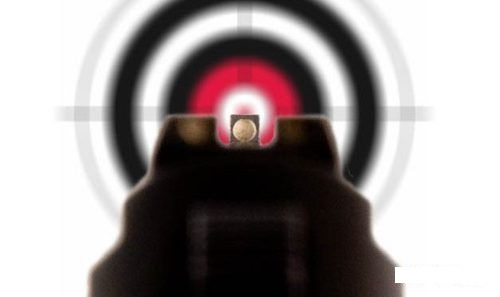
\includegraphics[width=6.7cm]{figure4.jpg}
        \caption{系统偏差}
        \label{figs:ShotExample2}
    \end{minipage}
\end{figure}


如果用以下式子去估计总体方差$\sigma^2$:
\begin{equation}
    S^2=\frac{1}{n}\sum\limits_{i-1}^n{(X_i-\bar{X})^2}
\end{equation}
会偏离靶心并产生偏差,这就是有偏的,这个偏差为$\frac{1}{n}\sigma^2$,
如图4,这种偏差就像瞄准镜歪了,属于系统误差,就此而言,无偏估计要好于有偏估计。


\subsection{有效性}
如图\ref{figs:effective},打靶的时候,右边的成绩肯定更优秀:
\begin{figure}[ht]
    \centering
    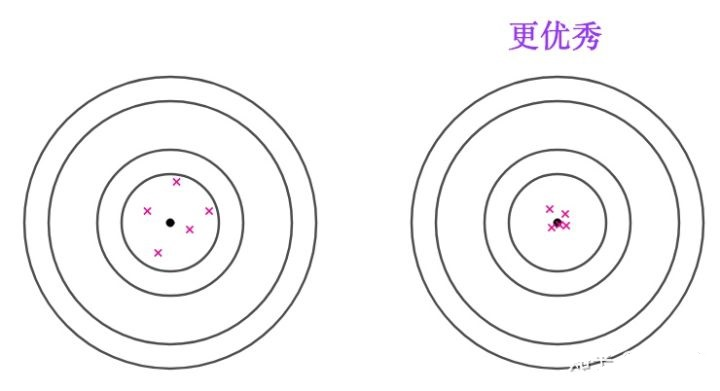
\includegraphics[width=10cm]{figure6.jpg}
    \caption{有效性示意图}
    \label{figs:effective}
\end{figure}
进行估计的时候,也是估计量越靠近目标,效果越好,这个靠近可以用方差来衡量。
另外,如图\ref{figs:effectiveOfbias}有效估计和偏差性是不相关的,无论是有偏估计还是无偏估计,
均可产生有效估计(方差更小)。
\begin{figure}[ht]
    \centering
    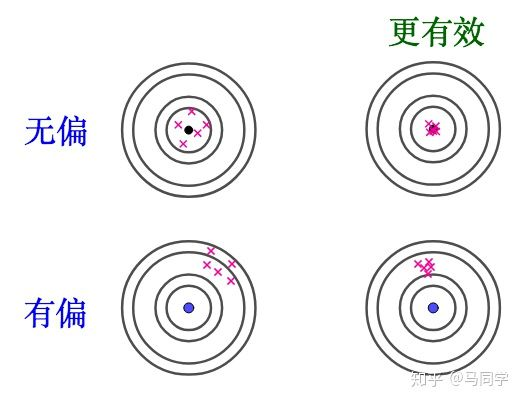
\includegraphics[width=10cm]{figure7.jpg}
    \caption{无偏和有偏下的有效性}
    \label{figs:effectiveOfbias}
\end{figure}
\par
举个例子,从$N(\mu,\sigma^2)$中抽出10个样本:
\begin{equation}
    \{x_1,x_2,\dots,x_n\}
\end{equation}
下面两个都是无偏估计量:
\begin{equation}
    T_1=\frac{x_1+x_3+2x_{10}}{4}, T_2=\frac{1}{10}\sum\limits_{i=1}^{10}{x_i}
\end{equation}
但是后者比前者方差小,后者更有效。并且实际系统中不一定非要选无偏估计量,如图\ref{figs:biasAndEffective}
\begin{figure}[ht]
    \centering
    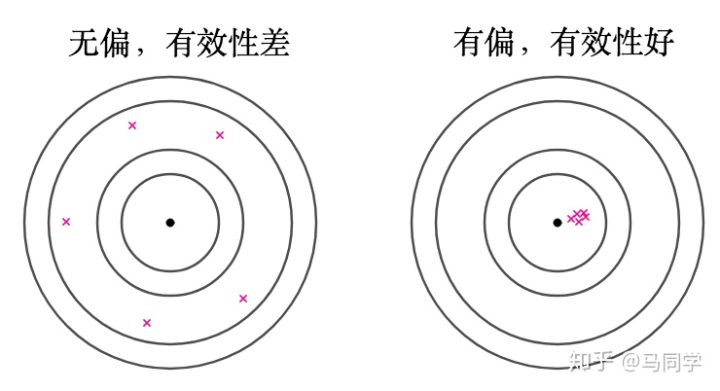
\includegraphics[width=10cm]{figure8.jpg}
    \caption{无偏性和有效性例子}
    \label{figs:biasAndEffective}
\end{figure}
如果能接受点误差,选择右边这个估计量更好。

\subsection{一致性}
如前所述,如果用以下式子去估计方差$\sigma^2$:
\begin{equation}
    S^2=\frac{1}{n}\sum\limits_{i-1}^n{(X_i-\bar{X})^2}
\end{equation}
会有一个偏差$\frac{1}{n}\sigma^2$,可以看到,随着采样个数$n$的增加,
这个偏差会越来越小。那么这个估计量就是“一致的”。如果样本数量够多,其实
这种“有偏”但是“一致'的估计量也是可以选的。
\subsection{总结}
在共视的Mapping中,由于固定历史帧,优化滑窗内的关键帧,导致的“有偏”估计,但是由于
前端vio能够提供无偏且一致的初值,会提升后端共视非线性优化的“有效性”,而且最终使得
SLAM能有一个比较精确的输出。

\section{非线性系统可观性分析}
\subsection{Lie Derivative}
在介绍Lie Derivative之前,先需要以下一些概念。\par

(1)向量函数$f(\textbf{x}):\mathbb{R}^n\rightarrow\mathbb{R}^n$(从$\textbf{x}\in\mathbb{R}^n$
映射到$f(\textbf{x})\in\mathbb{R}^n$),叫做$\mathbb{R}^n$里的向量场(Vector field)。
如果进一步,向量函数$f$具有连续偏导,而且是任意阶的偏导,那么我们说$f$是光滑向量场
(Smooth Vector field)。\par

(2)光滑标量函数$h(\textbf{x}):\mathbb{R}^n\rightarrow\mathbb{R}$(从$\textbf{x}\in\mathbb{R}^n$映射到
$h(\textbf{x})\in\mathbb{R}$的函数)的Gradient由一个行向量$\nabla{h}=\frac{\partial{h}}{\partial{\textbf{x}}}$
表示,其中$\textbf{x}\in\mathbb{R}^n$。所以我们要记住,Gradient是标量对向量的求导,
其结果是个行向量。光滑向量场$f(\textbf{x})$的Jacobian由一个$n\times{n}$的矩阵$\nabla{f}=\frac{\partial{f}}{\partial{\textbf{x}}}$,
其中矩阵的第一行就是$\nabla{f_1}=\frac{\partial{f_1}}{\partial{\textbf{x}}}$,就是刚刚定义的光滑标量函数$f_1$
(列向量$f$的第一个元素)的Gradient,而我们知道Gradient是行向量。以此类推Jacobian的第$i$行
应该为$\nabla{f_i}=\frac{\partial{f_i}}{\partial{\textbf{x}}}$。那么基于以上几个定义,我们就可以用来定义
Lie Derivative。\par

(3)Lie Derivative的定义:光滑标量函数$h(\textbf{x}):\mathbb{R}^n\rightarrow\mathbb{R}$相对于光滑向量场
$f(\textbf{x}):\mathbb{R}^n\rightarrow\mathbb{R}$的Lie Derivative由一个标量函数
$L_\textbf{f}h=\nabla{h}\textbf{f}=\frac{\partial{h}}{\partial{\textbf{x}}}\textbf{f}$表示,
其中$\frac{\partial{h}}{\partial{\textbf{x}}}$就是标量函数$h(\textbf{x})$的Gradient,
是个行向量。行向量$\frac{\partial{h}}{\partial{\textbf{x}}}$乘以向量场$f(\textbf{x})\in\mathbb{R}^n$,
其结果正好是个标量,所以$L_\textbf{f}h=\nabla{h}\textbf{f}=\frac{\partial{h}}{\partial{\textbf{x}}}f$
是个标量。\par

(4)如果$g(\textbf{x}):\mathbb{R}^n\rightarrow\mathbb{R}^n$是另一个向量场,由于刚刚计算的Lie Derivative:$L_\textbf{f}h$是个标量,
它又可以跟$g(\textbf{x})$算出一个Lie Derivative,表示为
$L_\textbf{g}L_\textbf{f}h=L_\textbf{g}(L_\textbf{f}h)=\nabla(L_\textbf{f}h)g=\frac{\partial(L_\textbf{f}h)}{\partial{\textbf{x}}}g
=\frac{\partial({\frac{\partial{h}}{\partial{\textbf{x}}}f)}}{\partial{\textbf{x}}}g$,
当然同样地,算出来$L_\textbf{g}L_\textbf{f}h$的结果依然是个标量。以此类推,可以一直搞下去。
于是我们有标量行数$h(\textbf{x}):\mathbb{R}^n\rightarrow\mathbb{R}$的0阶Lie Derivative,表示为
$L_\textbf{f}^0h=h$,是它本身。标量函数$h(\textbf{x}):\mathbb{R}^n\rightarrow\mathbb{R}$的第$i$阶
Lie Derivative为$L_\textbf{f}^ih=L_\textbf{f}(L_\textbf{f}^{i-1}h)=\nabla(L_{\textbf{f}}^{i-1}h)f=\frac{\partial(L_{\textbf{f}}^{i-1}h)}{\partial{\textbf{x}}}\textbf{f}$。\par
(5)总结一下,Lie Derivative与一般的Derivate的区别是,Lie Derivative是定义在两个函数$h$和$f$之间的,
它俩都是向量$\textbf{x}$的函数,标量行数$h$对$\textbf{x}$的Gradient乘以$f(\textbf{x})$,它们通过共同的
$\textbf{x}$联系起来的。一般的Derivative是某个函数对$\textbf{x}$定义的。举个例子,对于单输出非线性系统:
\begin{equation}
\begin{aligned}
    &\dot{\textbf{x}}=f(\textbf{x})\\
    &y=h(\textbf{x})
\end{aligned}
\end{equation}
我们有$\dot{y}=\frac{\partial{h}}{\partial{\textbf{x}}}\dot{\textbf{x}}=\frac{\partial{h}}{\partial{\textbf{x}}}f(\textbf{x})=L_\textbf{f}h$,
$\ddot{y}=\frac{\partial(L_\textbf{f}h)}{\partial{\textbf{x}}}\dot{\textbf{x}}=\frac{\partial(L_{\textbf{f}}h)}{\partial{\textbf{x}}}f(\textbf{x})=L_{\textbf{f}}^{2}h$

\subsection{非线性系统的Lie Derivative和可观矩阵}
考虑连续非线性系统:
\begin{equation}\label{eqs:nonlinearsys1}
    \begin{aligned}
    &\dot{\textbf{x}}=\textbf{f}_0(\textbf{x})+\sum\limits_{i=1}^{l}\textbf{f}_{i}(\textbf{x})\textbf{u}_i\\
    &\textbf{z}=\textbf{h}(\textbf{x})
    \end{aligned}
\end{equation}
其中控制输入$\textbf{u}=\left[u_1,u_2,\ldots, u_l\right]^T$,状态量$\textbf{x}=\left[x_1,x_2.\ldots,x_m\right]^T$,
状态过程模型表示为向量函数$\textbf{f}_i,i=0,1,\ldots,l$。$\left[3\right]$

\par
为了分析系统的可观性,以及在现有的测量下状态量各个方向的可观性,我们计算系统的Lie Derivative。定义测量函数$\textbf{h}$的零阶Lie Derivative
为其自身:
\begin{equation}
    \mathcal{L}^0\textbf{h}=\textbf{h}(\textbf{x})
\end{equation}
由Lie Derivative的定义,测量函数$\textbf{h}$不同阶的Lie Derivative由$\mathcal{L}^0\textbf{h}$循环计算得到。
其中,由第$i$阶Lie Derivative,$\mathcal{L}^i\textbf{h}$和状态过程函数$\textbf{f}_j$可计算得到测量函数的
第$i+1$阶Lie Derivative $\mathcal{L}_{\textbf{f}_j}^{i+1}\textbf{h}$:
\begin{equation}
    \mathcal{L}_{\textbf{f}_j}^{i+1}\textbf{h}=\nabla\mathcal{L}^i\textbf{h}\cdot\textbf{f}_j
\end{equation}
其中$\nabla\mathcal{L}^i\textbf{h}$为第$i$阶Lie Derivative的生成空间:
\begin{equation}
    \nabla\mathcal{L}^i\textbf{h}=\left[\frac{\partial\mathcal{L}^i\textbf{h}}{\partial{x_1}},
    \frac{\partial\mathcal{L}^i\textbf{h}}{\partial{x_2}},\dots,
    \frac{\partial\mathcal{L}^i\textbf{h}}{\partial{x_m}}
    \right]
\end{equation}
\par

由给定的观测信息,为了分析在哪些方向上是可观的,我们检查测量函数各阶Lie Derivative的生成空间,且定义可观矩阵为
\begin{equation}
    \mathcal{O}=
    \left[ \begin{array}{c}
        \nabla\mathcal{L}^0\textbf{h}\\
        \nabla\mathcal{L}_{\textbf{f}_i}^{1}\textbf{h}\\
        \nabla\mathcal{L}_{\textbf{f}_i\textbf{f}_j}^{2}\textbf{h}\\
        \nabla\mathcal{L}_{\textbf{f}_i\textbf{f}_j\textbf{f}_k}^{3}\textbf{h}\\
        \vdots
    \end{array}\right]
\end{equation}
其中$i,j,k=1,2,\dots,l$。为了证明系统是可观的,需要证明$\mathcal{O}$的若干行组成的子矩阵是列满秩的
(full colum rank)。相反的,为了证明系统是非完全可观的,且找出不可观的方向,则需要证明:
(a)矩阵$\mathcal{O}$中的无限多行,均可表示为矩阵$\mathcal{O}^\prime$行向量的线性组合,其中$\mathcal{O}\prime$
的行向量来自于$\mathcal{O}$;
(b)求解矩阵$\mathcal{O}\prime$的零空间,即可得到系统不可观的方向。尽管条件(b)可以直接求解得到,但是条件(a)很难
找到。
\par
{\color{red}注意:由Lie Derivative的定义可知,Lie Derivative是光滑标量函数$h(\textbf{x})$对向量$\textbf{x}$求生成空间(偏导数),
得到向量$\frac{\partial{h}}{\partial\textbf{x}}$后,再乘以光滑向量场$\textbf{f}(\textbf{x})$(向量),得到一个新的标量。
因此,如果$h(\textbf{x})$为向量,则应看作多个标量元素;如果$\textbf{f}(\textbf{x})$为矩阵,则应看作多个列向量,再计算Lie Derivative。}

\subsection{非线性系统可观性分析}
通过上面介绍可知,要分析非线性系统的可观性,是非常有挑战的,因为要计算具有无限行组成的可观矩阵的零空间。
但是论文中提出了一种方法,使可观性分析变得容易,将可观矩阵分解为两个矩阵相乘:一个满秩的无限行矩阵和一个
非满秩的有限行矩阵。下面将通过计算一系列关于状态变量$\textbf{x}$的基函数,来达到分解可观矩阵的目的。
\par
首先给出定理,
\par
\textbf{Theorem1:} 假设存在非线性变换$\mathbf{\beta(x)}=\left[\mathbf{\beta_1(x)}^T,\dots,\mathbf{\beta_t(x)}^T\right]^T$,
这些基均是关于状态变量$\textbf{x}$的函数,总共有$t$个,且满足如下条件:
\par
(C1)$\mathbf{\beta_1(x)}=\mathbf{h(x)}$;
\par
(C2)$\frac{\partial{\mathbf{\beta}}}{\partial{\textbf{x}}}\cdot\textbf{f}_i(\textbf{x}),i=0,1,\dots,l$是关于$\mathbf{\beta}$的函数;
\par
(C3)定义一个可观的非线性系统:
\begin{equation}\label{eqs:nonlinearsys2}
    \left\{ \begin{array}{l}
        \dot{\mathbf{\beta}}=\frac{\partial\mathbf{\beta}}{\partial\textbf{x}}\frac{\partial\textbf{x}}{\partial t}
            =\frac{\partial\mathbf{\beta}}{\partial\textbf{x}}\dot{\mathbf{x}}
            =\textbf{g}_0(\mathbf{\beta})+\sum_{i=1}^{l}{\textbf{g}_i(\mathbf{\beta})\textbf{u}_i}\\
        \textbf{z}=\textbf{h}=\mathbf{\beta}_1
    \end{array}\right.
\end{equation}
其中,$\textbf{g}_i(\mathbf{\beta})=\frac{\partial{\mathbf{\beta}}}{\partial{\textbf{x}}}\textbf{f}_i(\textbf{x}),i=0,1,\dots,l$。
\par
根据以上假设条件,则有以下两条结论:
\par
($\romannumeral1$)可观矩阵$\mathcal{O}$可被分解为:
\begin{equation}
    \mathcal{O}=\Xi\cdot\mathbf{B}
\end{equation}
其中$\Xi$为系统(\ref{eqs:nonlinearsys2})的可观矩阵,且$\mathbf{B}\triangleq\frac{\partial{\mathbf{\beta}}}{\partial{\textbf{x}}}$。
\par
($\romannumeral2$)$null(\mathcal{O})=null(\mathbf{B})$
\par
证明结论($\romannumeral1$):
根据链式法则,Lie Derivative $\nabla\mathcal{L}^i\textbf{h}$的生成空间可表示为,
\begin{equation}
    \nabla\mathcal{L}^i\textbf{h}=\frac{\partial\mathcal{L}^i\textbf{h}}{\partial{\textbf{x}}}
    =\frac{\partial\mathcal{L}^i\textbf{h}}{\partial\mathcal{\mathbf{\beta}}}\frac{\partial\mathbf{\beta}}{\partial{\textbf{x}}}
\end{equation}
因此,系统(\ref{eqs:nonlinearsys1})的可观矩阵$\mathcal{O}$可被分解为:
\begin{equation}
    \mathcal{O}
    =\left[ \begin{array}{c}
        \nabla\mathcal{L}^0\textbf{h}\\
        \nabla\mathcal{L}_{\textbf{f}_i}^{1}\textbf{h}\\
        \nabla\mathcal{L}_{\textbf{f}_i\textbf{f}_j}^{2}\textbf{h}\\
        \nabla\mathcal{L}_{\textbf{f}_i\textbf{f}_j\textbf{f}_k}^{3}\textbf{h}\\
        \vdots
    \end{array}\right]
    =\left[ \begin{array}{c}
        \frac{\partial\mathcal{L}^0\textbf{h}}{\partial\mathbf{\beta}}\\
        \frac{\partial\mathcal{L}^1_{\textbf{f}_i}\textbf{h}}{\partial\mathbf{\beta}}\\
        \frac{\partial\mathcal{L}^2_{\textbf{f}_i\textbf{f}_j}\textbf{h}}{\partial\mathbf{\beta}}\\
        \frac{\partial\mathcal{L}^3_{\textbf{f}_i\textbf{f}_j\textbf{f}_k}\textbf{h}}{\partial\mathbf{\beta}}\\
        \vdots
    \end{array}\right]\frac{\partial\mathbf{\beta}}{\partial\textbf{x}}
    =\Xi\cdot\textbf{B}
\end{equation}
接下来证明矩阵$\Xi$是系统(\ref{eqs:nonlinearsys2})的可观矩阵。
\par
为区分系统(\ref{eqs:nonlinearsys1})和系统(\ref{eqs:nonlinearsys2})的各阶Lie Derivative,
利用符号$\mathcal{J}$表示系统(\ref{eqs:nonlinearsys2})的Lie Derivative。
系统(\ref{eqs:nonlinearsys2})的零阶Lie Derivative的生成空间表示为:
\begin{equation}
    \nabla\mathcal{J}^0\textbf{h}=\frac{\partial\textbf{h}}{\partial\mathbf{\beta}}
    =\frac{\partial\mathcal{L}^0\textbf{h}}{\partial\mathbf{\beta}}
\end{equation}
该零阶生成空间即为矩阵$\Xi$的第一行块矩阵。
\par
利用$\nabla\mathcal{J}^i\textbf{h}=\frac{\partial\mathcal{L}^i\textbf{h}}{\partial\mathbf{\beta}}$表示矩阵$\Xi$
的$i$行Lie Derivative的生成空间,则第$i+1$行的生成空间$\nabla\mathcal{J}_{\textbf{g}_j}^{i+1}\textbf{h}$(状态过程函数为$\textbf{g}_j$)
可表示为
\begin{equation}
    \begin{array}{c}
        \nabla\mathcal{J}_{\textbf{g}_j}^{i+1}\textbf{h}=\frac{\partial\mathcal{J}_{\textbf{g}_j}^{i+1}\textbf{h}}{\partial\mathbf{\beta}}
        =\frac{\partial\nabla\mathcal{J}^i\textbf{h}\cdot\textbf{g}_j}{\partial\mathbf{\beta}}
        =\frac{\partial({\frac{\partial\mathcal{L}^i\textbf{h}}{\partial\mathbf{\beta}}}\cdot{{\frac{\partial\mathbf{\beta}}{\partial\textbf{x}}}{\textbf{f}_j}(\textbf{x})})}{\partial\mathbf{\beta}}
        =\frac{\partial({\frac{\partial\mathcal{L}^i\textbf{h}}{\partial{\textbf{x}}}}\cdot{\textbf{f}_j(\textbf{x})})}{\partial\mathbf{\beta}}
        =\frac{\partial\mathcal{L}_{\textbf{f}_j}^{i+1}\textbf{h}}{\partial\mathbf{\beta}}
    \end{array}
\end{equation}
因此,矩阵$\Xi$的每一行矩阵块,为系统(\ref{eqs:nonlinearsys2})的各阶Lie Derivative的生成空间,即矩阵$\Xi$是系统(\ref{eqs:nonlinearsys2})的可观矩阵。
\par
证明结论(\romannumeral2):由于$\mathcal{O}=\Xi\textbf{B}$,则有$null(\mathcal{O})=null(\textbf{B})+null(\Xi)\cap{range(\textbf{B})}$$\left[2\right]$,
另外,由于假设条件(C3)系统(\ref{eqs:nonlinearsys2})是可观的,即可观矩阵$\Xi$为列满秩(full column rank),
则有$null(\mathcal{O})=null(\textbf{B})$。至此,由假设条件(C1)、(C2)和(C3)得到的结论(\romannumeral1)和(\romannumeral2)证毕。
\par
由\textbf{Theorem1}可知,为了分析一个系统的不可观方向,首先需要找到一些基函数(basis functions)满足条件(C1)和(C2),并且需要证明
矩阵$\Xi$是列满秩(full column rank),即满足条件(C3)。当着三个条件满足后,则系统(\ref{eqs:nonlinearsys1})的不可观方向分析转换成求解
矩阵$\textbf{B}$的零空间。由于矩阵$\textbf{B}_I$是有限维的,因此求解零空间很容易。

\section{VI-SLAM系统可观性分析}
\subsection{系统概述}
在该系统中,四元数表示旋转采用JPL形式。坐标系约定:全局坐标系用$G$表示,Camera坐标系用$C$表示,
IMU坐标系用$I$表示,地图点用$f$表示;相机、IMU和地图点表示在某个坐标系下,则该坐标系符号写在对应变量符号的左上角,
变量标识写在变量符号的右下角,例如$\sideset{^G}{}{\mathop{\mathbf{p}_{I}}}$表示IMU系(body系)原点在全局坐标系中的位置(平移),
$\sideset{^G}{}{\mathop{\textbf{v}_{I}}}$表示IMU系在全局坐标系下的速度,$\sideset{^I}{}{\mathop{\textbf{q}_{G}}}$表示从全局坐标系
旋转到IMU系的单位四元数,由于采用JPL形式,旋转均是由$G$系到$I$系旋转,与Hamilton表示方式相反;$\sideset{^G}{}{\mathop{\textbf{p}_{f_i}}}$
表示第$i$个地图点在$G$系下的坐标。
\par
状态变量包含位姿、速度、Bias和地图点:
\begin{equation}
    \textbf{x}=\left[\sideset{^I}{}{\mathop{\textbf{q}_{G}^{T}}},
    \sideset{}{}{\mathop{\textbf{b}_{g}^{T}}},
    \sideset{^G}{}{\mathop{\textbf{v}_{I}^{T}}},
    \sideset{}{}{\mathop{\textbf{b}_{a}^{T}}},
    \sideset{^G}{}{\mathop{\textbf{p}_{I}^{T}}}|
    \sideset{^G}{}{\mathop{\textbf{p}_{f_1}^{T}}},
    \dots,
    \sideset{^G}{}{\mathop{\textbf{p}_{f_N}^{T}}}
    \right]^T
    =\left[\textbf{x}_{s}^{T} | \textbf{x}_{m}^{T}\right]^T
\end{equation}
其中$\textbf{x}_{s}^{T}$和$\textbf{x}_{m}^{T}$分别表示$16\times 1$维传感器状态和$3N\times 1$维地图点状态。
\par
连续系统状态模型:
\begin{equation}
    \sideset{^I}{}{\mathop{\dot{\mathbf{q}}_{G}(t)}}=\frac{1}{2}\mathbf{\Omega}(\sideset{^I}{}{\mathop{\omega(t)}})\sideset{^I}{}{\mathop{\textbf{q}_{G}(t)}}
\end{equation}
\begin{equation}
    \sideset{^G}{}{\mathop{\dot{\mathbf{p}}_{I}(t)}}=\sideset{^G}{}{\mathop{\textbf{v}_{I}(t)}}
\end{equation}
\begin{equation}
    \sideset{^G}{}{\mathop{\dot{\mathbf{v}}_{I}(t)}}=\sideset{^G}{}{\mathop{\textbf{a}_{I}(t)}}
\end{equation}
\begin{equation}
    \dot{\mathbf{b}}_{g}(t)=\textbf{n}_{wg}(t)
\end{equation}
\begin{equation}
    \dot{\mathbf{b}}_{a}(t)=\textbf{n}_{wa}(t)
\end{equation}
\begin{equation}
    \sideset{^G}{}{\mathop{\dot{\mathbf{p}}_{f_i}(t)}}=\textbf{0}_{3\times 1},i=1,\dots,N
\end{equation}
其中,
\begin{equation}
    \Omega(\omega)=\left[\begin{array}{cc}
        -\lfloor{\mathbf{\omega}}\rfloor_{\times} &\mathbf{\omega}\\
        -\mathbf{\omega}^T &\textbf{0}
    \end{array}\right]
\end{equation}
\begin{equation}
    \lfloor{\mathbf{\omega}}\rfloor_{\times}=\triangleq 
    \left[\begin{array}{ccc}
        0 &-\omega_3 &\omega_2\\
        \omega_3 &0 &-\omega_1\\
        -\omega_2 &\omega_1 &0
    \end{array}\right]
\end{equation}
\par
陀螺仪测量$\sideset{^I}{}{\mathop{\mathbf{\omega}_m}}$和加速度计测量$\sideset{^I}{}{\mathop{\mathbf{a}_m}}$模型为:
\begin{equation}
    \sideset{^I}{}{\mathop{\mathbf{\omega}_{m}(t)}}=\sideset{^I}{}{\mathop{\mathbf{\omega}(t)}}
    +\textbf{b}_{g}(t)+\textbf{n}_{g}(t)
\end{equation}
\begin{equation}
    \sideset{^I}{}{\mathop{\mathbf{a}_{m}(t)}}=\textbf{C}(\sideset{^I}{}{\mathop{\mathbf{q}_{G}(t)}})
    (\sideset{^G}{}{\mathop{\mathbf{a}_{I}(t)}}-\sideset{^G}{}{\mathop{\mathbf{g}}})
    +\textbf{b}_{a}(t)+\textbf{n}_{a}(t)
\end{equation}
其中$\textbf{C}(\mathbf{q})$表示四元数对应的选择矩阵。
\par
对于上述连续状态模型,在当前时刻的估计量处线性展开,并求期望,得到状态估计的传递模型:
\begin{equation}\label{eqs:sysmodel21}
    \sideset{^I}{}{\mathop{\dot{\hat{\mathbf{q}}}_{G}(t)}}=\frac{1}{2}\mathbf{\Omega}(\sideset{^I}{}{\mathop{\hat{\omega}(t)}})\sideset{^I}{}{\mathop{\hat{\mathbf{q}}_{G}(t)}}
\end{equation}
\begin{equation}\label{eqs:sysmodel22}
    \sideset{^G}{}{\mathop{\dot{\hat{\mathbf{p}}}_{I}(t)}}=\sideset{^G}{}{\mathop{\hat{\mathbf{v}}_{I}(t)}}
\end{equation}
\begin{equation}\label{eqs:sysmodel23}
    \sideset{^G}{}{\mathop{\dot{\hat{\mathbf{v}}}_{I}(t)}}=\textbf{C}^{T}(\sideset{^I}{}{\mathop{\hat{\mathbf{q}}_{G}(t)}})
    \sideset{^I}{}{\mathop{\hat{\mathbf{a}}(t)}}+\sideset{^G}{}{\mathop{\mathbf{g}}}
\end{equation}
\begin{equation}\label{eqs:sysmodel24}
    \dot{\mathbf{b}}_{g}(t)=\textbf{0}_{3\times 1}
\end{equation}
\begin{equation}\label{eqs:sysmodel25}
    \dot{\mathbf{b}}_{a}(t)=\textbf{0}_{3\times 1}
\end{equation}
\begin{equation}\label{eqs:sysmodel26}
    \sideset{^G}{}{\mathop{\dot{\hat{\mathbf{p}}}_{f_i}(t)}}=\textbf{0}_{3\times 1},i=1,\dots,N
\end{equation}
其中$\sideset{^I}{}{\mathop{\hat{\mathbf{a}}(t)}}=\sideset{^I}{}{\mathop{\mathbf{a}_{m}(t)}}-\hat{\mathbf{b}}_{a}(t)$,
$\sideset{^I}{}{\mathop{\hat{\mathbf{\omega}}(t)}}=\sideset{^I}{}{\mathop{\mathbf{\omega}_{m}(t)}}-\hat{\mathbf{b}}_{g}(t)$
\par
根据误差状态(error state)的定义$\tilde{\mathbf{x}}=\mathbf{x}-\hat{\mathbf{x}}$有:
\begin{equation}
    \tilde{\mathbf{x}}=\left[\sideset{^I}{}{\mathop{\delta{\mathbf{\theta}}_{G}^{T}}},
    \sideset{}{}{\mathop{\tilde{\mathbf{b}}_{g}^{T}}},
    \sideset{^G}{}{\mathop{\tilde{\textbf{v}}_{I}^{T}}},
    \sideset{}{}{\mathop{\tilde{\textbf{b}}_{a}^{T}}},
    \sideset{^G}{}{\mathop{\tilde{\textbf{p}}_{I}^{T}}}|
    \sideset{^G}{}{\mathop{\tilde{\textbf{p}}_{f_1}^{T}}},
    \dots,
    \sideset{^G}{}{\mathop{\tilde{\textbf{p}}_{f_N}^{T}}}
    \right]^T
    =\left[\tilde{\textbf{x}}_{s}^{T} | \tilde{\textbf{x}}_{m}^{T}\right]^T
\end{equation}
则有线性连续误差状态方程,
\begin{equation}
    \dot{\tilde{\mathbf{x}}}=\left[\begin{array}{cc}
        \textbf{F}_{s} &\textbf{0}_{15\times 3N}\\
        \textbf{0}_{3N\times 15} &\textbf{0}_{3N}
    \end{array}\right]\tilde{\textbf{x}}
    +\left[\begin{array}{c}
        \textbf{G}_{s}\\
        \textbf{0}_{3N\times 12}
    \end{array}\right]\textbf{n}
    =\textbf{F}_{c}\tilde{\textbf{x}}+\textbf{G}_{c}\textbf{n}
\end{equation}
其中,
\begin{equation}
    \textbf{n}=\left[\textbf{n}_{g}^{T}, \textbf{n}_{wg}^{T}, \textbf{n}_{a}^{T}, \textbf{n}_{wa}^{T}\right]^T
\end{equation}
\begin{equation}
    \textbf{F}_{s}=\left[\begin{array}{ccccc}
        -\lfloor{\hat{\mathbf{\omega}}}\rfloor_{\times} &-\textbf{I}_{3} &\textbf{0}_{3} &\textbf{0}_{3} &\textbf{0}_{3}\\
        \textbf{0}_{3} &\textbf{0}_{3} &\textbf{0}_{3} &\textbf{0}_{3} &\textbf{0}_{3}\\
        -\textbf{C}^{T}(\sideset{^I}{}{\mathop{\hat{\mathbf{q}}_{G}}})\lfloor{\sideset{^I}{}{\mathop{\hat{\mathbf{a}}}}}\rfloor_{\times}
        &\textbf{0}_{3} &\textbf{0}_{3} &-\textbf{C}^{T}(\sideset{^I}{}{\mathop{\hat{\mathbf{q}}_{G}}}) &\textbf{0}_{3}\\
        \textbf{0}_{3} &\textbf{0}_{3} &\textbf{0}_{3} &\textbf{0}_{3} &\textbf{0}_{3}\\
        \textbf{0}_{3} &\textbf{0}_{3} &\textbf{I}_{3} &\textbf{0}_{3} &\textbf{0}_{3}
    \end{array}\right]
\end{equation}
\begin{equation}
    \textbf{G}_{s}=\left[\begin{array}{cccc}
        -\textbf{I}_{3} &\textbf{0}_{3} &\textbf{0}_{3} &\textbf{0}_{3}\\
        \textbf{0}_{3} &\textbf{I}_{3} &\textbf{0}_{3} &\textbf{0}_{3}\\
        \textbf{0}_{3} &\textbf{0}_{3} &-\textbf{C}^{T}(\sideset{^I}{}{\mathop{\hat{\mathbf{q}}_{G}}}) &\textbf{0}_{3}\\
        \textbf{0}_{3} &\textbf{0}_{3} &\textbf{0}_{3} &\textbf{I}_{3}\\
        \textbf{0}_{3} &\textbf{0}_{3} &\textbf{0}_{3} &\textbf{0}_{3}
    \end{array}\right]
\end{equation}
\begin{equation}
    \mathbb{E}\left[\mathbf{n}(t)\mathbf{n}^{T}(\tau)\right]=\textbf{Q}_{c}\delta(t-\tau)
\end{equation}

\par
接下来讨论离散形式的系统模型:假设陀螺仪信号$\sideset{^I}{}{\mathop{\mathbf{\omega}_{m}(t)}}$
和加速度计信号$\sideset{^I}{}{\mathop{\mathbf{a}_{m}(t)}}$采样间隔为$\delta{t}\triangleq t_{k+1}-t_{k}$,
每次采样后,系统估计状态的传递,利用公式(\ref{eqs:sysmodel21})-(\ref{eqs:sysmodel26})积分得到。
估计状态的协方差通过如下公式得到:
\begin{equation}
    \begin{array}{c}
    \dot{\Phi}_{k+1,k} = \mathbf{F}_{c}\Phi_{k+1,k}\\
    initial\ condition:\ \Phi_{k,k}=\mathbf{I}_{15+3N}
    \end{array}
\end{equation}
\begin{equation}
    \textbf{P}_{k+1|k}=\Phi_{k+1,k}\mathbf{P}_{k|k}\Phi_{k+1,k}^{T}+\textbf{Q}_{d,k}
\end{equation}
其中离散的系统噪声协方差矩阵$\textbf{Q}_{d,k}$通过如下积分计算,
\begin{equation}
    \textbf{Q}_{d,k}=\int_{t_k}^{t_{k+1}}\Phi(t_{k+1},\tau)\textbf{G}_{c}\textbf{Q}_{c}\textbf{G}_{c}^{T}
    \Phi^{T}(t_{k+1},\tau)d\tau
\end{equation}

\par
下面讨论视觉观测模型:为简化问题分析,假设只有一个地图点$\textbf{p}_{f_i}$,其对应相机测量$\textbf{z}_i$
为地图点$\sideset{^I}{}{\mathop{\textbf{p}_{f_i}}}$在图像平面上的投影,即有
\begin{equation}\label{eqs:visualmodel1}
    \textbf{z}_{i}=\frac{1}{p_z}\left[\begin{array}{c} p_x\\p_y\end{array}\right]+\eta_i
\end{equation}
其中
\begin{equation}\label{eqs:visualmodel2}
    \left[\begin{array}{c} p_x\\p_y\\p_z \end{array}\right]
        =\sideset{^I}{}{\mathop{\mathbf{p}_{f_i}}}
        =\textbf{C}(\sideset{^I}{}{\mathop{\mathbf{q}_{G}}})
        (\sideset{^G}{}{\mathop{\mathbf{p}_{f_i}}}-\sideset{^G}{}{\mathop{\mathbf{p}_I}})
\end{equation}
且$\eta_i$为协方差为$\textbf{R}_i$的高斯白噪声。注意:该视觉观察模型假设图像测量为归一化平面,且相机坐标系
和IMU坐标系重合,在实际中,相机和IMU之间存在内外参。
\par
视觉观测的误差模型表示为
\begin{equation}
    \tilde{\mathbf{z}}_{i}=\textbf{z}_{i}-\hat{\mathbf{z}}_{i} \simeq \textbf{H}_{i}\tilde{\textbf{x}}+\eta_{i}
\end{equation}
其中$\hat{\textbf{z}}=\textbf{h}(\hat{\textbf{x}})$是利用当前时刻估计状态$\hat{\textbf{x}}$通过模型(\ref{eqs:visualmodel1})-(\ref{eqs:visualmodel2})
计算得到,且视觉测量雅可比矩阵$\textbf{H}_{i}$为
\begin{equation}
    \textbf{H}_{i}=\textbf{H}_{c}
    \left[\textbf{H}_{\theta}\ \ \textbf{0}_{3\times 9}\ \ \textbf{H}_{p}\ \ |\ \ 
    \textbf{0}_{3}\dots\textbf{H}_{f_i}\dots\textbf{0}_{3}\right]
\end{equation}
其中
\begin{equation}
    \textbf{H}_{c}=\frac{\partial\textbf{h}}{\partial\sideset{^I}{}{\mathop{\textbf{p}_{f_i}}}}
    =\frac{1}{p_{z}^{2}}\left[\begin{array}{ccc}
    p_z &0 &-p_x\\
    0 &p_z &-p_y
    \end{array}\right]
\end{equation}
\begin{equation}
    \textbf{H}_{\theta}=\frac{\partial\sideset{^I}{}{\mathop{\textbf{p}_{f_i}}}}{\partial{\theta}}
    =\lfloor\textbf{C}(\sideset{^I}{}{\mathop{\textbf{q}_{G}}})
    (\sideset{^G}{}{\mathop{\textbf{p}_{f_i}}}-\sideset{^G}{}{\mathop{\textbf{p}_I}}) \rfloor_{\times}
\end{equation}
\begin{equation}
    \textbf{H}_{p}=\frac{\partial\sideset{^I}{}{\mathop{\textbf{p}_{f_i}}}}{\partial\sideset{^G}{}{\mathop{\textbf{p}_I}}}
    =-\textbf{C}(\sideset{^I}{}{\mathop{\textbf{q}_G}})
\end{equation}
\begin{equation}
    \textbf{H}_{f_i}=\frac{\partial\sideset{^I}{}{\mathop{\textbf{p}_{f_i}}}}{\partial\sideset{^G}{}{\mathop{\textbf{p}_{f_i}}}}
    =\textbf{C}(\sideset{^I}{}{\mathop{\textbf{q}_G}})
\end{equation}

\subsection{可观性分析}
为简化分析,将$I$系旋转用Cayley-Gibbs-Rodriguez(CGR)方式表示:$\sideset{^I}{}{\mathop{\textbf{s}_{G}}}$表示从$G$系到$I$系的旋转,且有
\begin{equation}
    \sideset{^I}{}{\mathop{\dot{\textbf{s}}_{G}(t)}}=\textbf{D}(\sideset{^I}{}{\mathop{\mathbf{\omega}(t)}}-\textbf{b}_{g}(t))
\end{equation}
其中$\textbf{D}\triangleq \frac{\partial\textbf{s}}{\partial\theta}=\frac{1}{2}(\textbf{I}_{3}+\lfloor\textbf{s}\rfloor_{\times}+\textbf{s}\textbf{s}^T)$。
因此,系统状态变量$\textbf{x}$可表示为
\begin{equation}
    \textbf{x}=\left[\sideset{^I}{}{\mathop{\textbf{s}_{G}}}\ \ \textbf{b}_{g}^{T}
    \ \ \sideset{^G}{}{\mathop{\textbf{v}_{I}^{T}}}\ \ \textbf{b}_{a}^{T}\ \ \sideset{^G}{}{\mathop{\textbf{p}_{I}^{T}}}
    \ \ \sideset{^G}{}{\mathop{\textbf{p}_{f}^{T}}}\right]^T
\end{equation}
另外,为简化书写,系统状态变量忽略坐标系标识,
\begin{equation}
    \textbf{x}=\left[\textbf{s}^T\ \ \textbf{b}_{g}^{T}\ \ \textbf{v}^{T}\ \ \textbf{b}_{a}^{T}
    \ \ \textbf{p}^{T}\ \ \textbf{p}_{f}^{T}\right]^T
\end{equation}
则有VI-SLAM状态模型可表示为
\begin{equation}
    \left[\begin{array}{c}
        \dot{\textbf{s}}\\\dot{\textbf{b}}_{g}\\\dot{\textbf{v}}\\
        \dot{\textbf{b}_{a}}\\\dot{\textbf{p}}\\\dot{\textbf{p}}_{f}
    \end{array}\right]
    =\left[\begin{array}{c}
        -\textbf{D}\textbf{b}_{g}\\\textbf{0}_{3\times 1}\\\textbf{g}-\textbf{C}^{T}\textbf{b}_{a}\\
        \textbf{0}_{3\times 1}\\\textbf{v}\\\textbf{0}_{3\times 1}
    \end{array}\right]
    +\left[\begin{array}{c}
        \textbf{D}\\\textbf{0}_{3}\\\textbf{0}_{3}\\\textbf{0}_{3}\\\textbf{0}_{3}\\\textbf{0}_{3}
    \end{array}\right]\mathbf{\omega}
    +\left[\begin{array}{c}
        \textbf{0}_{3}\\\textbf{0}_{3}\\\textbf{C}^{T}\\\textbf{0}_{3}\\\textbf{0}_{3}\\\textbf{0}_{3}
    \end{array}\right]\textbf{a}
\end{equation}
\begin{equation}
    \textbf{z}=\frac{1}{p_z}\left[\begin{array}{c} p_x\\p_y \end{array}\right]
\end{equation}
其中$\textbf{C}\triangleq\textbf{C}(\textbf{s})$,
$\left[\begin{array}{c} p_x\\p_y\\p_z \end{array}\right]=\sideset{^I}{}{\mathop{\textbf{p}_{f}}}
    =\textbf{C}\cdot(\textbf{p}_{f}-\textbf{p})$,且令
\begin{equation}
    \textbf{f}_{0}=\left[\begin{array}{c}
        -\textbf{D}\textbf{b}_{g}\\\textbf{0}_{3\times 1}\\\textbf{g}-\textbf{C}^{T}\textbf{b}_{a}\\
        \textbf{0}_{3\times 1}\\\textbf{v}\\\textbf{0}_{3\times 1}
    \end{array}\right],
    \textbf{f}_{1}=\left[\begin{array}{c}
        \textbf{D}\\\textbf{0}_{3}\\\textbf{0}_{3}\\\textbf{0}_{3}\\\textbf{0}_{3}\\\textbf{0}_{3}
    \end{array}\right],
    \textbf{f}_{2}=\left[\begin{array}{c}
        \textbf{0}_{3}\\\textbf{0}_{3}\\\textbf{C}^{T}\\\textbf{0}_{3}\\\textbf{0}_{3}\\\textbf{0}_{3}
    \end{array}\right]
\end{equation}

\par
接下来分析系统的可观性:首先根据\textbf{Theorem1}中的假设条件(C1)和(C2),找到系统的基函数(basis functions),其中直接根据条件(C1)
得到第一个基函数$\mathbf{\beta}_{1}=\textbf{z}=\textbf{h}(\textbf{x})$,
\begin{equation}
    \mathbf{\beta}_{1}\triangleq \textbf{h}(\textbf{x})=\frac{1}{p_z}
    \left[\begin{array}{c} p_x\\p_y \end{array}\right]
\end{equation}
然后循环计算条件(C2)中的$\frac{\partial\mathbf{\beta}_j}{\partial\textbf{x}}\cdot\textbf{f}_{i}$,
并寻找新的基函数$\mathbf{\beta}$,其中基函数有很多种选择,应当选择那些有明确物理意义的量作为基函数。
\par
计算基函数$\mathbf{\beta}_1$关于$\textbf{x}$的生成空间,
\begin{equation}
    \begin{array}{ll}\frac{\partial\mathbf{\beta}_1}{\partial\textbf{x}}
        &=\left[\frac{\partial\mathbf{\beta}_1}{\partial\mathbf{\theta}}\frac{\partial\mathbf{\theta}}{\partial\textbf{s}}
        \ \ \frac{\partial\mathbf{\beta}_1}{\partial\textbf{x}_{g}}\ \ \frac{\partial\mathbf{\beta}_1}{\partial\textbf{v}}
        \ \ \frac{\partial\mathbf{\beta}_1}{\partial\textbf{b}_{a}}\ \ \frac{\partial\mathbf{\beta}_1}{\partial\textbf{p}}
        \ \ \frac{\partial\mathbf{\beta}_1}{\partial\textbf{p}_f}\right]\\
        &=\frac{\partial\textbf{h}}{\partial\sideset{^I}{}{\mathop{\textbf{p}_{f}}}}
        \frac{\partial\sideset{^I}{}{\mathop{\textbf{p}_{f}}}}{\partial\textbf{x}}\\
        &=\left[\begin{array}{ccc}
            \frac{1}{p_z} &0 &-\frac{p_x}{p_z^2}\\
            0 &\frac{1}{p_z} &-\frac{p_y}{p_z^2}\end{array}\right]
            \left[\lfloor\sideset{^I}{}{\mathop{\textbf{p}_{f}}}\rfloor_{\times}\frac{\partial\mathbf{\theta}}{\partial\textbf{s}}
            \ \ \textbf{0}_3\ \ \textbf{0}_3\ \ \textbf{0}_3\ \ -\textbf{C}\ \ \textbf{C}
            \right]
    \end{array}
\end{equation}

\par
计算$\frac{\partial\mathbf{\beta}_1}{\partial\textbf{x}}\cdot\textbf{f}_0$:
\begin{equation}
    \begin{array}{ll}
        \frac{\partial\mathbf{\beta}_1}{\partial\textbf{x}}\cdot\textbf{f}_{0}
        &=\left[\begin{array}{ccc}
        \frac{1}{p_z} &0 &-\frac{p_x}{p_z^2}\\
        0 &\frac{1}{p_z} &-\frac{p_y}{p_z^2}\end{array}\right]
        (-\lfloor\sideset{^I}{}{\mathop{\textbf{p}_{f}}}\rfloor_{\times}\textbf{b}_{g}-\textbf{C}\textbf{v})\\
        &=\left[\textbf{I}_{2}\ \ -\mathbf{\beta}_{1}\right]
        (-\lfloor\left[\begin{array}{c} \mathbf{\beta}_1\\ 1 \end{array}\right]\rfloor_{\times}\textbf{b}_{g}-\frac{1}{p_z}\textbf{C}\textbf{v})
    \end{array}
\end{equation}
显然$\frac{\partial\mathbf{\beta}_1}{\partial\textbf{x}}\cdot\textbf{f}_0$没法表示成现有基函数$\{\mathbf{\beta}_1\}$的函数,
因此增加基函数:
\begin{eqnarray}
    \mathbf{\beta}_2\triangleq& \frac{1}{p_z}\\
    \mathbf{\beta}_3\triangleq& \textbf{C}\textbf{v}\\
    \mathbf{\beta}_4\triangleq& \textbf{b}_{g}
\end{eqnarray}
其中$\mathbf{\beta}_2$表示地图的逆深度,$\mathbf{\beta}_3$表示$I$系下的速度,$\mathbf{\beta}_4$表示陀螺仪bias,则有,
\begin{equation}
    \frac{\partial\mathbf{\beta}_1}{\partial\textbf{x}}\cdot\textbf{f}_{0}
    \triangleq\left[\textbf{I}_{2}\ \ -\mathbf{\beta}_{1}\right]
    (-\lfloor\left[\begin{array}{c} \mathbf{\beta}_1\\ 1 \end{array}\right]\rfloor_{\times}
        \mathbf{\beta}_4-\mathbf{\beta}_{2}\mathbf{\beta}_3)
\end{equation}

计算$\frac{\partial\mathbf{\beta}_1}{\partial\textbf{x}}\cdot\textbf{f}_1$:
\begin{equation}
    \begin{array}{ll}
        \frac{\partial\mathbf{\beta}_1}{\partial\textbf{x}}\cdot\textbf{f}_1
        &=\left[\begin{array}{ccc} \frac{1}{p_z}&0&-\frac{p_x}{p_z^2}\\
        0&\frac{1}{p_z}&-\frac{p_y}{p_z^2} \end{array}\right]
        \lfloor\sideset{^I}{}{\mathop{\textbf{p}_f}} \rfloor_{\times}\\
        &=\left[\begin{array}{cc} \textbf{I}_{2}\ \ -\mathbf{\beta}_{1} \end{array}\right]
        \lfloor\left[\begin{array}{c}\mathbf{\beta}_1\\1 \end{array}\right] \rfloor_{\times}
    \end{array}
\end{equation}
无需增加新的基函数。
\par
计算$\frac{\partial\mathbf{\beta}_1}{\partial\textbf{x}}\cdot\textbf{f}_2$:
\begin{equation}
    \frac{\partial\mathbf{\beta}_1}{\partial\textbf{x}}\cdot\textbf{f}_2=\textbf{0}_{2\times 1}
\end{equation}
无需增加新的基函数。

\par
计算基函数$\mathbf{\beta}_2$关于$\textbf{x}$的生成空间,
\begin{equation}
    \begin{array}{ll}\frac{\partial\mathbf{\beta}_2}{\partial\textbf{x}}
        &=\left[\frac{\partial\mathbf{\beta}_2}{\partial\mathbf{\theta}}\frac{\partial\mathbf{\theta}}{\partial\textbf{s}}
        \ \ \frac{\partial\mathbf{\beta}_2}{\partial\textbf{x}_{g}}\ \ \frac{\partial\mathbf{\beta}_2}{\partial\textbf{v}}
        \ \ \frac{\partial\mathbf{\beta}_2}{\partial\textbf{b}_{a}}\ \ \frac{\partial\mathbf{\beta}_2}{\partial\textbf{p}}
        \ \ \frac{\partial\mathbf{\beta}_2}{\partial\textbf{p}_f}\right]\\
        &=\frac{\partial\mathbf{\beta}_2}{\partial\sideset{^I}{}{\mathop{\textbf{p}_{f}}}}
        \frac{\partial\sideset{^I}{}{\mathop{\textbf{p}_{f}}}}{\partial\textbf{x}}\\
        &=-\frac{1}{p_z^2}\textbf{e}_{3}^{T}
            \left[\lfloor\sideset{^I}{}{\mathop{\textbf{p}_{f}}}\rfloor_{\times}\frac{\partial\mathbf{\theta}}{\partial\textbf{s}}
            \ \ \textbf{0}_3\ \ \textbf{0}_3\ \ \textbf{0}_3\ \ -\textbf{C}\ \ \textbf{C}
            \right]
    \end{array}
\end{equation}
其中$\textbf{e}_3$为$3\times 3$单位矩阵第三列:$\left[\textbf{e}_1\ \ \textbf{e}_2\ \ \textbf{e}_3\right]=\textbf{I}_3$。

\par
计算$\frac{\partial\mathbf{\beta}_2}{\partial\textbf{x}}\cdot\textbf{f}_0$:
\begin{equation}
    \begin{array}{ll}
        \frac{\partial\mathbf{\beta}_2}{\partial\textbf{x}}\cdot\textbf{f}_0
        &=-\frac{1}{p_z^2}\textbf{e}_{3}^{T}(-\lfloor\sideset{^I}{}{\mathop{\textbf{p}_{f}}}\rfloor_{\times}\textbf{b}_{g}-\textbf{Cv})\\
        &=-\mathbf{\beta}_{2}\textbf{e}_{3}^{T}(-\lfloor\left[\begin{array}{c}\mathbf{\beta}_1\\1 \end{array}\right] \rfloor_{\times}
            \mathbf{\beta}_{4}-\mathbf{\beta}_{2}\mathbf{\beta}_{3})
    \end{array}
\end{equation}
无需增加新的基函数。

\par
计算$\frac{\partial\mathbf{\beta}_2}{\partial\textbf{x}}\cdot\textbf{f}_1$:
\begin{equation}
    \begin{array}{ll}
        \frac{\partial\mathbf{\beta}_2}{\partial\textbf{x}}\cdot\textbf{f}_1
        &=-\frac{1}{p_z^2}\textbf{e}_{3}^{T}\lfloor\sideset{^I}{}{\mathop{\textbf{p}_{f}}}\rfloor_{\times}\\
        &=-\mathbf{\beta}_{2}\textbf{e}_{3}^{T}\lfloor\left[\begin{array}{c}\mathbf{\beta}_1\\1 \end{array}\right] \rfloor_{\times}
    \end{array}
\end{equation}
无需增加新的基函数。

\par
计算$\frac{\partial\mathbf{\beta}_2}{\partial\textbf{x}}\cdot\textbf{f}_2$:
\begin{equation}
    \frac{\partial\mathbf{\beta}_2}{\partial\textbf{x}}\cdot\textbf{f}_2=0
\end{equation}
无需增加新的基函数。

\par
计算基函数$\mathbf{\beta}_3$关于$\textbf{x}$的生成空间,
\begin{equation}
    \begin{array}{ll}\frac{\partial\mathbf{\beta}_3}{\partial\textbf{x}}
        &=\left[\frac{\partial\mathbf{\beta}_3}{\partial\mathbf{\theta}}\frac{\partial\mathbf{\theta}}{\partial\textbf{s}}
        \ \ \frac{\partial\mathbf{\beta}_3}{\partial\textbf{x}_{g}}\ \ \frac{\partial\mathbf{\beta}_3}{\partial\textbf{v}}
        \ \ \frac{\partial\mathbf{\beta}_3}{\partial\textbf{b}_{a}}\ \ \frac{\partial\mathbf{\beta}_3}{\partial\textbf{p}}
        \ \ \frac{\partial\mathbf{\beta}_3}{\partial\textbf{p}_f}\right]\\
        &=\left[\lfloor\textbf{Cv}\rfloor_{\times}\frac{\partial\mathbf{\theta}}{\partial\textbf{s}}
        \ \ \textbf{0}_3\ \ \textbf{C}\ \ \textbf{0}_3\ \ \textbf{0}_3\ \ \textbf{0}_3
        \right]
    \end{array}
\end{equation}

\par
计算$\frac{\partial\mathbf{\beta}_3}{\partial\textbf{x}}\cdot\textbf{f}_0$:
\begin{equation}
    \begin{array}{ll}
        \frac{\partial\mathbf{\beta}_3}{\partial\textbf{x}}\cdot\textbf{f}_0
        &=-\lfloor\textbf{Cv}\rfloor_{\times}\textbf{b}_{g}+\textbf{C}\ \textbf{g}-\textbf{b}_{a}\\
        &\triangleq -\lfloor\mathbf{\beta}_3\rfloor_{\times}\mathbf{\beta}_{4}+\mathbf{\beta}_{5}-\mathbf{\beta}_{6}
    \end{array}
\end{equation}
其中定义新的基函数:
\begin{equation}
    \mathbf{\beta}_5 \triangleq \textbf{C}\ \textbf{g}
\end{equation}
\begin{equation}
    \mathbf{\beta}_6 \triangleq \textbf{b}_{a}
\end{equation}
其中$\mathbf{\beta}_5$表示$I$系下的重力方向,$\mathbf{\beta}_6表示加速度计bias$。

\par
计算$\frac{\partial\mathbf{\beta}_3}{\partial\textbf{x}}\cdot\textbf{f}_1$:
\begin{equation}
    \frac{\partial\mathbf{\beta}_3}{\partial\textbf{x}}\cdot\textbf{f}_1
    =\lfloor\textbf{Cv}\rfloor_{\times}
\end{equation}
无需增加新的基函数。

\par
计算$\frac{\partial\mathbf{\beta}_3}{\partial\textbf{x}}\cdot\textbf{f}_2$:
\begin{equation}
    \frac{\partial\mathbf{\beta}_3}{\partial\textbf{x}}\cdot\textbf{f}_2=\textbf{I}_3
\end{equation}
无需增加新的基函数。

\par
计算基函数$\mathbf{\beta}_4$关于$\textbf{x}$的生成空间,
\begin{equation}
    \begin{array}{ll}\frac{\partial\mathbf{\beta}_4}{\partial\textbf{x}}
        &=\left[\frac{\partial\mathbf{\beta}_4}{\partial\mathbf{\theta}}\frac{\partial\mathbf{\theta}}{\partial\textbf{s}}
        \ \ \frac{\partial\mathbf{\beta}_4}{\partial\textbf{x}_{g}}\ \ \frac{\partial\mathbf{\beta}_4}{\partial\textbf{v}}
        \ \ \frac{\partial\mathbf{\beta}_4}{\partial\textbf{b}_{a}}\ \ \frac{\partial\mathbf{\beta}_4}{\partial\textbf{p}}
        \ \ \frac{\partial\mathbf{\beta}_4}{\partial\textbf{p}_f}\right]\\
        &=\left[\textbf{0}_3\ \ \textbf{I}_3\ \ \textbf{0}_3\ \ \textbf{0}_3\ \ \textbf{0}_3\ \ \textbf{0}_3\right]
    \end{array}
\end{equation}

\par
计算$\frac{\partial\mathbf{\beta}_4}{\partial\textbf{x}}\cdot\textbf{f}_0$:
\begin{equation}
    \frac{\partial\mathbf{\beta}_4}{\partial\textbf{x}}\cdot\textbf{f}_0=\textbf{0}_{3\times 1}
\end{equation}
无需增加新的基函数。

\par
计算$\frac{\partial\mathbf{\beta}_4}{\partial\textbf{x}}\cdot\textbf{f}_1$:
\begin{equation}
    \frac{\partial\mathbf{\beta}_4}{\partial\textbf{x}}\cdot\textbf{f}_1=\textbf{0}_{3\times 1}
\end{equation}
无需增加新的基函数。

\par
计算$\frac{\partial\mathbf{\beta}_4}{\partial\textbf{x}}\cdot\textbf{f}_2$:
\begin{equation}
    \frac{\partial\mathbf{\beta}_4}{\partial\textbf{x}}\cdot\textbf{f}_2=\textbf{0}_{3\times 1}
\end{equation}
无需增加新的基函数。


\par
计算基函数$\mathbf{\beta}_5$关于$\textbf{x}$的生成空间,
\begin{equation}
    \begin{array}{ll}\frac{\partial\mathbf{\beta}_5}{\partial\textbf{x}}
        &=\left[\frac{\partial\mathbf{\beta}_5}{\partial\mathbf{\theta}}\frac{\partial\mathbf{\theta}}{\partial\textbf{s}}
        \ \ \frac{\partial\mathbf{\beta}_5}{\partial\textbf{x}_{g}}\ \ \frac{\partial\mathbf{\beta}_5}{\partial\textbf{v}}
        \ \ \frac{\partial\mathbf{\beta}_5}{\partial\textbf{b}_{a}}\ \ \frac{\partial\mathbf{\beta}_5}{\partial\textbf{p}}
        \ \ \frac{\partial\mathbf{\beta}_5}{\partial\textbf{p}_f}\right]\\
        &=\left[\lfloor\textbf{C}\ \textbf{g}\rfloor_{\times}\frac{\partial\mathbf{\theta}}{\partial\textbf{s}}
        \ \ \textbf{0}_3\ \ \textbf{0}_3\ \ \textbf{0}_3\ \ \textbf{0}_3\ \ \textbf{0}_3\right]
    \end{array}
\end{equation}

\par
计算$\frac{\partial\mathbf{\beta}_5}{\partial\textbf{x}}\cdot\textbf{f}_0$:
\begin{equation}
    \frac{\partial\mathbf{\beta}_5}{\partial\textbf{x}}\cdot\textbf{f}_0
    =-\lfloor\textbf{C}\ \textbf{g}\rfloor_{\times}\textbf{b}_{g}
    =-\lfloor\mathbf{\beta}_5\rfloor_{\times}\mathbf{\beta}_4
\end{equation}
无需增加新的基函数。

\par
计算$\frac{\partial\mathbf{\beta}_5}{\partial\textbf{x}}\cdot\textbf{f}_1$:
\begin{equation}
    \frac{\partial\mathbf{\beta}_5}{\partial\textbf{x}}\cdot\textbf{f}_1
    =\lfloor\textbf{C}\ \textbf{g}\rfloor_{\times}
    =\lfloor\mathbf{\beta}_5\rfloor_{\times}
\end{equation}
无需增加新的基函数。

\par
计算$\frac{\partial\mathbf{\beta}_5}{\partial\textbf{x}}\cdot\textbf{f}_2$:
\begin{equation}
    \frac{\partial\mathbf{\beta}_5}{\partial\textbf{x}}\cdot\textbf{f}_2=\textbf{0}_{3\times 1}
\end{equation}
无需增加新的基函数。

\par
计算基函数$\mathbf{\beta}_6$关于$\textbf{x}$的生成空间,
\begin{equation}
    \begin{array}{ll}\frac{\partial\mathbf{\beta}_6}{\partial\textbf{x}}
        &=\left[\frac{\partial\mathbf{\beta}_6}{\partial\mathbf{\theta}}\frac{\partial\mathbf{\theta}}{\partial\textbf{s}}
        \ \ \frac{\partial\mathbf{\beta}_6}{\partial\textbf{x}_{g}}\ \ \frac{\partial\mathbf{\beta}_6}{\partial\textbf{v}}
        \ \ \frac{\partial\mathbf{\beta}_6}{\partial\textbf{b}_{a}}\ \ \frac{\partial\mathbf{\beta}_6}{\partial\textbf{p}}
        \ \ \frac{\partial\mathbf{\beta}_6}{\partial\textbf{p}_f}\right]\\
        &=\left[\textbf{0}_3\ \ \textbf{0}_3\ \ \textbf{0}_3\ \ \textbf{I}_3\ \ \textbf{0}_3\ \ \textbf{0}_3\right]
    \end{array}
\end{equation}

\par
计算$\frac{\partial\mathbf{\beta}_6}{\partial\textbf{x}}\cdot\textbf{f}_0$:
\begin{equation}
    \frac{\partial\mathbf{\beta}_6}{\partial\textbf{x}}\cdot\textbf{f}_0=\textbf{0}_{3\times 1}
\end{equation}
无需增加新的基函数。

\par
计算$\frac{\partial\mathbf{\beta}_6}{\partial\textbf{x}}\cdot\textbf{f}_1$:
\begin{equation}
    \frac{\partial\mathbf{\beta}_6}{\partial\textbf{x}}\cdot\textbf{f}_1=\textbf{0}_{3\times 1}
\end{equation}
无需增加新的基函数。

\par
计算$\frac{\partial\mathbf{\beta}_6}{\partial\textbf{x}}\cdot\textbf{f}_2$:
\begin{equation}
    \frac{\partial\mathbf{\beta}_6}{\partial\textbf{x}}\cdot\textbf{f}_2=\textbf{0}_{3\times 1}
\end{equation}
无需增加新的基函数。

\par
至此,总共定义6个基函数:
\begin{eqnarray}
    \mathbf{\beta}_1 =& \textbf{h}(\textbf{x})\\
    \mathbf{\beta}_2 =& \frac{1}{p_z}\\
    \mathbf{\beta}_3 =& \textbf{Cv}\\
    \mathbf{\beta}_4 =& \textbf{b}_g\\
    \mathbf{\beta}_5 =& \textbf{Cg}\\
    \mathbf{\beta}_6 =& \textbf{b}_a& 
\end{eqnarray}

\par
根据$\textbf{Theorem1}$中条件(C3),由基函数构建的非线性系统为:
\begin{equation}
    \dot{\mathbf{\beta}}=\frac{\partial\mathbf{\beta}}{\partial\textbf{x}}\frac{\partial\textbf{x}}{\partial t}
    =\frac{\partial\mathbf{\beta}}{\partial\textbf{x}}\dot{\mathbf{x}}
    =\frac{\partial\mathbf{\beta}}{\partial\textbf{x}}(\textbf{f}_{0}+\textbf{f}_{1}\mathbf{\omega}+\textbf{f}_{2}\mathbf{a})
    =\textbf{g}_0+\textbf{g}_{1}\mathbf{\omega}+\textbf{g}_{2}\textbf{a}
\end{equation}
即有
\begin{equation}\label{eqs:nonlinearsys3}
    \left[\begin{array}{c}\dot{\mathbf{\beta}}_1\\ \dot{\mathbf{\beta}}_2\\
    \dot{\mathbf{\beta}}_3\\ \dot{\mathbf{\beta}}_4\\
    \dot{\mathbf{\beta}}_5\\ \dot{\mathbf{\beta}}_6
    \end{array}\right]
    =\left[\begin{array}{c}\bar{\bar{\mathbf{\beta}}}_{1}(-\lfloor\bar{\mathbf{\beta}}_{1}\rfloor_{\times}\mathbf{\beta}_{4}
    -\mathbf{\beta}_{2}\mathbf{\beta}_3) \\
    \mathbf{\beta}_{2}\textbf{e}_{3}^{T}(\lfloor\bar{\mathbf{\beta}}_1\rfloor_{\times}\mathbf{\beta}_{4}
    +\mathbf{\beta}_{2}\mathbf{\beta}_{3})\\
    -\lfloor\mathbf{\beta}_3\rfloor_{\times}\mathbf{\beta}_{4}+\mathbf{\beta}_5-\mathbf{\beta}_6\\
    \textbf{0}_{3\times 1}\\
    -\lfloor\mathbf{\beta}_5\rfloor_{\times}\mathbf{\beta}_4\\\textbf{0}_{3\times 1}
    \end{array}\right]
    +\left[\begin{array}{c} \bar{\bar{\mathbf{\beta}}}_{1}\lfloor\bar{\mathbf{\beta}}_{1}\rfloor_{\times}\\
    -\mathbf{\beta}_{2}\textbf{e}_{3}^{T}\lfloor\bar{\mathbf{\beta}}_{1}\rfloor_{\times}\\
    \lfloor\mathbf{\beta}_3\rfloor_{\times}\\\textbf{0}_3\\\lfloor\mathbf{\beta}_5\rfloor_{\times}\\
    \textbf{0}_3
    \end{array}\right]\mathbf{\omega}
    +\left[\begin{array}{c}\textbf{0}_{2\times 3}\\\textbf{0}_{1\times 3}\\\textbf{I}_3\\
    \textbf{0}_3\\\textbf{0}_3\\\textbf{0}_3 \end{array}\right]\textbf{a}
\end{equation}
\begin{equation}
    \textbf{z}=\textbf{h}(\textbf{x})=\mathbf{\beta}_1
\end{equation}
其中$\bar{\mathbf{\beta}}_{1}=\left[\mathbf{\beta}_{1}^{T}\ \ 1\right]^T$,
$\bar{\bar{\mathbf{\beta}}}_{1}=\left[\textbf{I}_{2}\ \ -\mathbf{\beta}_{1}\right]$。

\par
下面讨论基于基函数$\mathbf{\beta}$的系统(\ref{eqs:nonlinearsys3})可观性,即检查是否满足$\textbf{Theorem1}$中的条件(\textbf{C3}):
系统(\ref{eqs:nonlinearsys3})的可观矩阵$\Xi$是否为列满秩。由可观矩阵的定义可知,矩阵$\Xi$是一个无数行的矩阵,
但是为了证明该矩阵为列满秩,可以选取它的子矩阵$\Xi'$来分析,如果$\Xi'$是列满秩,则$\Xi$也是列满秩。
选取Lie Derivative集合$\mathcal{L}$计算可观子矩阵$\Xi'$:
\begin{equation}
    \mathcal{L}=\{\mathcal{L}^{0}\textbf{h},\mathcal{L}_{\textbf{g}_{0}\textbf{g}_{13}\textbf{g}_{21}}^{3}\textbf{h},
    \mathcal{L}_{\textbf{g}_{0}}^{1}\textbf{h}, \mathcal{L}_{\textbf{g}_{0}\textbf{g}_{13}\textbf{g}_{13}}^{3}\textbf{h},
    \mathcal{L}_{\textbf{g}_{0}\textbf{g}_{0}\textbf{g}_{21}}^{3}\textbf{h},
    \mathcal{L}_{\textbf{g}_{0}\textbf{g}_{0}}^{2}\textbf{h},
    \mathcal{L}_{\textbf{g}_{0}\textbf{g}_{0}\textbf{g}_{13}}^{3}\textbf{h},
    \mathcal{L}_{\textbf{g}_{0}\textbf{g}_{0}\textbf{g}_{0}}^{3}\textbf{h}\}
\end{equation}
其中$\textbf{g}_{ij}$表示矩阵$\textbf{g}_{i}$的第$j$列,即$\textbf{g}_{ij}=\textbf{g}_{i}\textbf{e}_{j}$,
$\textbf{e}_{j}$为单位矩阵的第$j$列。

\par
计算Lie Derivative集合$\mathcal{L}$关于基函数$\mathbf{\beta}$的生成空间,得到可观矩阵$\Xi'$:
\begin{equation}
    \Xi'=\left[\begin{array}{c}
    \frac{\partial{\mathcal{L}^{0}}\textbf{h}}{\partial{\mathbf{\beta}}}\\
    \frac{\partial{\mathcal{L}^{3}_{\textbf{g}_{0}\textbf{g}_{13}\textbf{g}_{21}}\textbf{h}}}{\partial{\mathbf{\beta}}}\\
    \frac{\partial{\mathcal{L}^{1}_{\textbf{g}_0}}\textbf{h}}{\partial{\mathbf{\beta}}}\\
    \frac{\partial{\mathcal{L}^{3}_{\textbf{g}_{0}\textbf{g}_{13}\textbf{g}_{13}}\textbf{h}}}{\partial{\mathbf{\beta}}}\\
    \frac{\partial{\mathcal{L}^{3}_{\textbf{g}_{0}\textbf{g}_{0}\textbf{g}_{21}}\textbf{h}}}{\partial{\mathbf{\beta}}}\\
    \frac{\partial{\mathcal{L}^{2}_{\textbf{g}_{0}\textbf{g}_{0}}\textbf{h}}}{\partial{\mathbf{\beta}}}\\
    \frac{\partial{\mathcal{L}^{3}_{\textbf{g}_{0}\textbf{g}_{0}\textbf{g}_{13}}\textbf{h}}}{\partial{\mathbf{\beta}}}\\
    \frac{\partial{\mathcal{L}^{3}_{\textbf{g}_{0}\textbf{g}_{0}\textbf{g}_{0}}\textbf{h}}}{\partial{\mathbf{\beta}}}\\
    \end{array}\right]
    =\left[\begin{array}{ccc} \textbf{I}_{3\times 3}& \textbf{0}_{3\times 6}& \textbf{0}_{3\times 6}\\
    \textbf{0}_{1\times 3}& \textbf{0}_{1\times 6}& \textbf{0}_{1\times 6}\\
    \textbf{X}_{6\times 3}& {\Psi}_{6\times 6}& \textbf{0}_{6\times 6}\\
    \textbf{Y}_{6\times 3}& \mathbf{Z}_{6\times 6}& {\Theta}_{6\times 6}
    \end{array}\right]
\end{equation}
其中第二行块矩阵为零,舍弃掉后得到新观测矩阵:
\begin{equation}
    \Xi''=\left[\begin{array}{ccc} \textbf{I}_{3\times 3}& \textbf{0}_{3\times 6}& \textbf{0}_{3\times 6}\\
        \textbf{X}_{6\times 3}& {\Psi}_{6\times 6}& \textbf{0}_{6\times 6}\\
        \textbf{Y}_{6\times 3}& \mathbf{Z}_{6\times 6}& {\Theta}_{6\times 6}
        \end{array}\right]
\end{equation}
为证明矩阵$\Xi''$为列满秩,只需证明矩阵$\Psi$和$\Theta$为满秩矩阵。

\par
矩阵$\Psi$具体为:
\begin{equation}
\Psi=\left[\begin{array}{cccccc} 
    -\beta_{21}&0&\beta_{11}\beta_{21}&-\beta_{11}\beta_{12}&\beta_{11}^{2}+1&-\beta_{12}\\
    0&-\beta_{21}&\beta_{12}\beta_{21}&-\beta_{12}^{2}-1&\beta_{11}\beta_{12}&-\beta_{11}\\
    \beta_{21}&0&-\beta_{11}\beta_{21}&4\beta_{11}\beta_{12}&2\beta_{12}^{2}-2\beta_{11}^{2}&\beta_{12}\\
    0&\beta_{21}&-\beta_{12}\beta_{21}&2\beta_{12}^{2}-2\beta_{11}^{2}&-4\beta_{11}\beta_{12}&-\beta_{11}\\
    0&0&-\beta_{21}^{2}&2\beta_{12}\beta_{21}&-4\beta_{11}\beta_{21}&0\\
    0&0&0&0&-2\beta_{12}\beta_{21}&-2\beta_{21}
\end{array}\right]
\end{equation}
其中$\beta_{ij}$表示第$i$个基函数$\mathbf{\beta}_i$的第$j$个元素。
通过检查矩阵$\Psi$的行列式,
\begin{equation}
    det(\Psi)=-4\beta_{21}^{5}(\beta_{11}^{2}+\beta_{12}^{2}-1)(2\beta_{11}^{2}+2\beta_{12}^{2}+1)
    =-4\frac{1}{p_z^5}(\frac{p_x^2}{p_z^2}+\frac{p_y^2}{p_z^2}-1)(2\frac{p_x^2}{p_z^2}+2\frac{p_y^2}{p_z^2}+1)
\end{equation}
由于$p_z\not=0$且$2\frac{p_x^2}{p_z^2}+2\frac{p_y^2}{p_z^2}+1\geqslant 1$,因此矩阵$\Psi$的行列式唯一可能为零
的情况为$\frac{p_x^2}{p_z^2}+\frac{p_y^2}{p_z^2}-1=0$,即:所有地图点的视觉观测,位于图像归一化平面的单位圆上。
这中情况在实际中是不可能事件,因为控制输入是随着时间任意变化的。因而矩阵$\Psi$一般而言是满秩的。

\par
矩阵$\Theta$具体为:
\begin{equation}
    \Theta=\left[\begin{array}{cccccc} 
        -\beta_{21}&0&\beta_{11}\beta_{21}&\beta_{21}&0&-\beta_{11}\beta_{21}\\
        0&-\beta_{21}&\beta_{12}\beta_{21}&0&\beta_{21}&-\beta_{12}\beta_{21}\\
        0&-\beta_{21}&\beta_{12}\beta_{21}&0&0&-\beta_{12}\beta_{21}\\
        \beta_{21}&0&-\beta_{11}\beta_{21}&0&0&\beta_{11}\beta_{21}\\
        \Theta_{5,1}&\Theta_{5,2}&\Theta_{5,3}&\Theta_{5,4}&\Theta_{5,5}&\Theta_{5,6}\\
        \Theta_{6,1}&\Theta_{6,2}&\Theta_{6,3}&\Theta_{6,4}&\Theta_{6,5}&\Theta_{6,6}
    \end{array}\right]
\end{equation}
其中,
\begin{equation}
    \Theta_{5,1}=-2\beta_{21}(\beta_{11}\beta_{42}-\beta_{12}\beta_{41}+\beta_{21}\beta_{33})
    -\beta_{21}(2\beta_{11}\beta_{42}-\beta_{12}\beta_{41}+\beta_{21}\beta_{33})-2\beta_{11}\beta_{21}\beta_{42}
\end{equation}
\begin{equation}
    \Theta_{5,2}=2\beta_{21}\beta_{43}+\beta_{21}(\beta_{43}+\beta_{11}\beta_{41})+2\beta_{11}\beta_{21}\beta_{41}
\end{equation}
\begin{equation}
    \begin{array}{ll}
        \Theta_{5,3}=&2\beta_{21}(\beta_{42}-\beta_{21}\beta_{31}-\beta_{12}\beta_{43}+
        \beta_{11}(\beta_{11}\beta_{42}-\beta_{12}\beta_{41}+\beta_{21}\beta_{33}))-2\beta_{21}\beta_{42}\\
        &-\beta_{21}^{2}(\beta_{31}-\beta_{11}\beta_{33})-\beta_{12}\beta_{21}(\beta_{43}+\beta_{11}\beta_{41})
        +2\beta_{11}\beta_{21}(\beta_{11}\beta_{42}-\beta_{12}\beta_{41}+\beta_{21}\beta_{33})\\
        &+\beta_{11}\beta_{21}(2\beta_{11}\beta_{42}-\beta_{12}\beta_{41}+\beta_{21}\beta_{33})
    \end{array}
\end{equation}
\begin{equation}
    \Theta_{5,4}=2\beta_{21}(\beta_{11}\beta_{42}-\beta_{12}\beta_{41}+\beta_{21}\beta_{33})
    +\beta_{21}(2\beta_{11}\beta_{42}-\beta_{12}\beta_{41}+\beta_{21}\beta_{33})+\beta_{11}\beta_{21}\beta_{42}
\end{equation}
\begin{equation}
    \Theta_{5,5}=-\beta_{21}\beta_{43}-\beta_{21}(\beta_{43}+\beta_{11}\beta_{41})-\beta_{11}\beta_{21}\beta_{41}
\end{equation}
\begin{equation}
    \begin{array}{ll}
    \Theta_{5,6}=&\beta_{21}^{2}(\beta_{31}-\beta_{11}\beta_{33})+\beta_{21}\beta_{42}-2\beta_{21}(\beta_{42}-\beta_{21}\beta_{31}\\
    &-\beta_{12}\beta_{43}+\beta_{11}(\beta_{11}\beta_{42}-\beta_{12}\beta_{41}+\beta_{21}\beta_{33}))
    +\beta_{12}\beta_{21}(\beta_{43}+\beta_{11}\beta_{41})-2\beta_{11}\beta_{21}\\
    &(\beta_{11}\beta_{42}-\beta_{12}\beta_{41}+\beta_{21}\beta_{33})
    -\beta_{11}\beta_{21}(2\beta_{11}\beta_{42}-\beta_{12}\beta_{41}+\beta_{21}\beta_{33})
    \end{array}
\end{equation}
\begin{equation}
    \Theta_{6,1}=-2\beta_{21}\beta_{43}-\beta_{21}(\beta_{43}+\beta_{12}\beta_{42})-2\beta_{12}\beta_{21}\beta_{42}
\end{equation}
\begin{equation}
    \Theta_{6,2}=2\beta_{12}\beta_{21}\beta_{41}-\beta_{21}(\beta_{11}\beta_{42}-2\beta_{12}\beta_{41}+\beta_{21}\beta_{33})
    -2\beta_{21}(\beta_{11}\beta_{42}-\beta_{12}\beta_{41}+\beta_{21}\beta_{33})
\end{equation}
\begin{equation}
    \begin{array}{ll}
    \Theta_{6,3}=&2\beta_{21}\beta_{41}-\beta_{21}^{2}(\beta_{32}-\beta_{12}\beta_{33})
    -2\beta_{21}(\beta_{41}+\beta_{21}\beta_{32}-\beta_{11}\beta_{43}\\
    &-\beta_{12}(\beta_{11}\beta_{42}-\beta_{12}\beta_{41}+\beta_{21}\beta_{33}))\\
    &+\beta_{11}\beta_{21}(\beta_{43}+\beta_{12}\beta_{41})+2\beta_{12}\beta_{21}
    (\beta_{11}\beta_{42}-\beta_{12}\beta_{41}+\beta_{21}\beta_{33})\\
    &+\beta_{12}\beta_{21}(\beta_{11}\beta_{42}-2\beta_{12}\beta_{41}+\beta_{21}\beta_{33})
    \end{array}
\end{equation}
\begin{equation}
    \Theta_{6,4}=\beta_{21}\beta_{43}+\beta_{21}(\beta_{43}+\beta_{12}\beta_{42})+\beta_{12}\beta_{21}\beta_{42}
\end{equation}
\begin{equation}
    \Theta_{6,5}=2\beta_{21}(\beta_{11}\beta_{42}-\beta_{12}\beta_{41}+\beta_{21}\beta_{33})
    +\beta_{21}(\beta_{11}\beta_{42}-2\beta_{12}\beta_{41}+\beta_{21}\beta_{33})-\beta_{12}\beta_{21}\beta_{41}
\end{equation}
\begin{equation}
    \begin{array}{ll}
        \Theta_{6,6} = &\beta_{21}^{2}(\beta_{32}-\beta_{12}\beta_{33})-\beta_{21}\beta_{41}
        +2\beta_{21}(\beta_{41}+\beta_{21}\beta_{32}-\beta_{11}\beta_{43}\\
        &-\beta_{12}(\beta_{11}\beta_{42}-\beta_{12}\beta_{41}+\beta_{21}\beta_{33}))
        -\beta_{11}\beta_{21}(\beta_{43}+\beta_{12}\beta_{42})\\
        &-2\beta_{12}\beta_{21}(\beta_{11}\beta_{42}-\beta_{12}\beta_{41}+\beta_{21}\beta_{33})
        -\beta_{12}\beta_{21}(\beta_{11}\beta_{42}-2\beta_{12}\beta_{41}+\beta_{21}\beta_{33})
    \end{array}
\end{equation}
检查矩阵$\Theta$的行列式:
\begin{equation}
    \begin{array}{ll}
        det(\Theta)=&3\beta_{21}^{7}(\beta_{11}\beta_{33}\beta_{41}-\beta_{32}\beta_{42}-\beta_{31}\beta_{41}
        +\beta_{12}\beta_{33}\beta_{42})\\
        &=3\beta_{21}^{7}\left[\beta_{11}\beta_{33}-\beta_{31}, \beta_{12}\beta_{33}-\beta_{32}\right]
        \left[\begin{array}{c}
            \beta_{41}\\\beta_{42}
        \end{array}\right]
    \end{array}
\end{equation}
其中$\beta_{21}=\frac{1}{p_z}\not=0$;$\beta_4=\textbf{b}_{g}\not=0$;
由于$\beta_1=\textbf{h}$,以及$\beta_3=\textbf{Cv}$,则有
\begin{equation}
    \left[\beta_{11}\beta_{33}-\beta_{31}, \beta_{12}\beta_{33}-\beta_{32}\right]^T=\textbf{A}\beta_3
\end{equation}
因为$\beta_3\not=\textbf{0}_{3\times 1}$(相机移动),并且矩阵$\textbf{A}$为列满秩,则有$\textbf{A}\beta_1\not=0$。
最后检查
\begin{equation}
    \begin{array}{c}
        \left[\beta_{11}\beta_{33}-\beta_{31}, \beta_{12}\beta_{33}-\beta_{32}\right]
        \left[\begin{array}{c}
            \beta_{41}\\\beta_{42}
        \end{array}\right]=0\\
        \Leftrightarrow \left[\beta_{41},\beta_{42}\right]\textbf{A}\beta_3=0\\
    \Leftrightarrow \textbf{A}\beta_3=
        \lambda\left[\begin{array}{c}\beta_{42}\\-\beta_{41} \end{array}\right],\lambda\in\mathbb{R}
    \end{array}
\end{equation}
从上式可看出,对于给定的$\beta_{41}$和$\beta_{42}$,由于$\beta_1$是时变的,因此矩阵$\textbf{A}$
将$\beta_3=\textbf{Cv}$限定在特定的流形上,这在实际的任意控制输入系统中,是不存在的。因此有
\begin{equation}
    \left[\beta_{11}\beta_{33}-\beta_{31}, \beta_{12}\beta_{33}-\beta_{32}\right]
    \left[\begin{array}{c}
        \beta_{41}\\\beta_{42}
    \end{array}\right]\not=0
\end{equation}
因而矩阵$\Theta$一般而言是满秩的。

\par
至此,矩阵$\Psi$和$\Theta$均为满秩,对于可观矩阵$\Xi''$,利用左上角的单位矩阵,
高斯消元消去矩阵$\textbf{X}_{6\times 3}$和$\textbf{Y}_{6\times 3}$;利用中间的$\Psi$消去
矩阵$\textbf{Z}_{6\times 6}$,即可得到新的可观矩阵,
\begin{equation}
    \Xi'''=\left[\begin{array}{ccc} \textbf{I}_{3\times 3}& \textbf{0}_{3\times 6}& \textbf{0}_{3\times 6}\\
        \textbf{0}_{6\times 3}& {\Psi}_{6\times 6}& \textbf{0}_{6\times 6}\\
        \textbf{0}_{6\times 3}& \mathbf{0}_{6\times 6}& {\Theta}_{6\times 6}
        \end{array}\right]
\end{equation}
由于矩阵$\Psi$和$\Theta$均为满秩,非主对角线元素均为零,所以有矩阵$\Xi'''$为满秩,
进而可知可观矩阵$\Xi$为列满秩。

\par
下面讨论$\mathcal{O}=\Xi\textbf{B}$中的$\textbf{B}$矩阵,通过分析矩阵$\textbf{B}$的零空间,
得到系统不可观的情况。通过堆叠基函数$\beta$对状态变量$\textbf{x}$的偏导,得到,
\begin{equation}
    \textbf{B}=\left[\begin{array}{ccccc}
    \mathbf{\xi}&\textbf{0}_3&\textbf{0}_3&\textbf{0}_3&\textbf{0}_3\\
    \textbf{0}_3&\textbf{I}_3&\textbf{0}_3&\textbf{0}_3&\textbf{0}_3\\
    \textbf{0}_3&\textbf{0}_3&\textbf{I}_3&\textbf{0}_3&\textbf{0}_3\\
    \textbf{0}_3&\textbf{0}_3&\textbf{0}_3&\textbf{I}_3&\textbf{0}_3\\
    \textbf{0}_3&\textbf{0}_3&\textbf{0}_3&\textbf{0}_3&\textbf{I}_3
    \end{array}\right]
    \left[\begin{array}{cccccc}
        \lfloor\sideset{^I}{}{\mathop{\textbf{p}_f}}\rfloor_{\times}\frac{\partial\mathbf{\theta}}{\partial\textbf{s}}&\textbf{0}_3&\textbf{0}_3&\textbf{0}_3&-\textbf{C}&\textbf{C}\\
        \lfloor\textbf{Cv}\rfloor_{\times}\frac{\partial\mathbf{\theta}}{\partial\textbf{s}}&\textbf{0}_3&\textbf{C}&\textbf{0}_3&\textbf{0}_3&\textbf{0}_3\\
        \textbf{0}_3&\textbf{I}_3&\textbf{0}_3&\textbf{0}_3&\textbf{0}_3&\textbf{0}_3\\
        \lfloor\textbf{Cg}\rfloor_{\times}\frac{\partial\mathbf{\theta}}{\partial\textbf{s}}&\textbf{0}_3&\textbf{0}_3&\textbf{0}_3&\textbf{0}_3&\textbf{0}_3\\
        \textbf{0}_3&\textbf{0}_3&\textbf{0}_3&\textbf{I}_3&\textbf{0}_3&\textbf{0}_3
    \end{array}\right]
    \triangleq \textbf{B}_{1}\textbf{B}_{2}
\end{equation}
其中,
\begin{equation}
    \mathbf{\xi}=\left[\begin{array}{ccc}
        \frac{1}{p_z}&0&-\frac{p_x}{p_z^2}\\
        0&\frac{1}{p_z}&-\frac{p_y}{p_z^2}\\
        0&0&-\frac{1}{p_z^2}
    \end{array}\right]
\end{equation}
显然矩阵$\textbf{B}_1$满秩,则只需分析$15\times 18$矩阵$\textbf{B}_2$的零空间。
直观得到并验证,下列矩阵为$\textbf{B}_2$的右零空间(right null space),
\begin{equation}
    \textbf{N}_R=\left[\begin{array}{cc}
        \textbf{0}_3&\frac{\partial\textbf{s}}{\partial\mathbf{\theta}}\textbf{Cg}\\
        \textbf{0}_3&\textbf{0}_3\\
        \textbf{0}_3&-\lfloor\textbf{v}\rfloor_{\times}\textbf{g}\\
        \textbf{0}_3&\textbf{0}_{3\times 1}\\
        \textbf{I}_3&-\lfloor\textbf{p}\rfloor_{\times}\textbf{g}\\
        \textbf{I}_3&-\lfloor\textbf{p}_f\rfloor_{\times}\textbf{g}
    \end{array}\right]
\end{equation}
接下来证明矩阵$\textbf{B}_2$无其它右零空间向量:通过证明矩阵$\textbf{B}_2$的左零空间(left null space)
只有1维,即有$15\times 18$矩阵$\textbf{B}_2$的秩为14,进而矩阵$\textbf{B}_2$的右零空间有$18-14=4$维。
假设左零空间为$\textbf{N}_L=\left[\textbf{N}_1,\textbf{N}_2,\textbf{N}_3,\textbf{N}_4,\textbf{N}_5\right]$,则有
\begin{equation}
    \textbf{0}=\left[\textbf{N}_1,\textbf{N}_2,\textbf{N}_3,\textbf{N}_4,\textbf{N}_5\right]
    \left[\begin{array}{cccccc}
        \lfloor\sideset{^I}{}{\mathop{\textbf{p}_f}}\rfloor_{\times}\frac{\partial\mathbf{\theta}}{\partial\textbf{s}}&\textbf{0}_3&\textbf{0}_3&\textbf{0}_3&-\textbf{C}&\textbf{C}\\
        \lfloor\textbf{Cv}\rfloor_{\times}\frac{\partial\mathbf{\theta}}{\partial\textbf{s}}&\textbf{0}_3&\textbf{C}&\textbf{0}_3&\textbf{0}_3&\textbf{0}_3\\
        \textbf{0}_3&\textbf{I}_3&\textbf{0}_3&\textbf{0}_3&\textbf{0}_3&\textbf{0}_3\\
        \lfloor\textbf{Cg}\rfloor_{\times}\frac{\partial\mathbf{\theta}}{\partial\textbf{s}}&\textbf{0}_3&\textbf{0}_3&\textbf{0}_3&\textbf{0}_3&\textbf{0}_3\\
        \textbf{0}_3&\textbf{0}_3&\textbf{0}_3&\textbf{I}_3&\textbf{0}_3&\textbf{0}_3
    \end{array}\right]
\end{equation}
由矩阵$\textbf{B}_2$的第2列和第4列可知,$\textbf{N}_3\textbf{I}_3=\textbf{0}$和$\textbf{N}_5\textbf{I}_3=\textbf{0}$,
则有$\textbf{N}_3=\textbf{0}$,$\textbf{N}_5=\textbf{0}$;由矩阵$\textbf{B}_2$的第3列和第5、6列可知,
$\textbf{N}_1\textbf{C}=\textbf{0}$和$\textbf{N}_2\textbf{C}=\textbf{0}$,由于旋转矩阵$\textbf{C}$为满秩,则有
$\textbf{N}_1=\textbf{0}$,$\textbf{N}_2=\textbf{0}$;因此,只有向量$\textbf{N}_4$为左零空间的非零项,由矩阵$\textbf{B}_2$
的第1列可知,
\begin{equation}
    \textbf{N}_{4}\lfloor\textbf{Cg}\rfloor_{\times}\frac{\partial\mathbf{\theta}}{\partial\textbf{s}}=\textbf{0}
\end{equation}
由于矩阵$\frac{\partial\mathbf{\theta}}{\partial\textbf{s}}$为满秩,则有
\begin{equation}
    \textbf{N}_4=\pm(\textbf{Cg})^T
\end{equation}
因此矩阵$\textbf{B}_2$有左零空间,
\begin{equation}
    \textbf{N}_L=\left[\textbf{0}_{1\times 3},\textbf{0}_{1\times 3},\textbf{0}_{1\times 3},(\textbf{Cg})^T,\textbf{0}_{1\times 3}\right]
\end{equation}
且其只有1维。至此,可知矩阵$\textbf{B}_2$有且仅有右零空间$\textbf{N}_R$。

\par
接下来讨论右零空间$\textbf{N}_R$每一维对应的物理意义,即有哪些量是不可观的。
令$\textbf{N}_R=span\left[\textbf{n}_{1},\textbf{n}_{2},\textbf{n}_{3},\textbf{n}_{4}\right]$,
利用$\textbf{n}_{1},\textbf{n}_{2},\textbf{n}_{3},\textbf{n}_{4}$对状态变量
$\textbf{x}=\left[\sideset{^I}{}{\mathop{\textbf{s}_{G}}}\ \ \textbf{b}_{g}^{T}
\ \ \sideset{^G}{}{\mathop{\textbf{v}_{I}^{T}}}\ \ \textbf{b}_{a}^{T}\ \ \sideset{^G}{}{\mathop{\textbf{p}_{I}^{T}}}
\ \ \sideset{^G}{}{\mathop{\textbf{p}_{f}^{T}}}\right]^T$进行微小扰动,
通过观察$\textbf{x}$中哪些量会变化,则对应的量即为不可观的。
\par
首先利用$\textbf{n}_{1},\textbf{n}_{2},\textbf{n}_{3}$对$\textbf{x}$施加扰动,
\begin{equation}
    \textbf{x}'=\textbf{x}+c_1\textbf{n}_1+c_2\textbf{n}_2+c_3\textbf{n}_3
\end{equation}
\begin{equation}
    \delta\textbf{x}=c_1\textbf{n}_1+c_2\textbf{n}_2+c_3\textbf{n}_3
\end{equation}
对应于$\sideset{^G}{}{\mathop{\textbf{p}_{I}^{T}}}$和$\sideset{^G}{}{\mathop{\textbf{p}_{f}^{T}}}$变化,
即$\textbf{n}_1,\textbf{n}_2,\textbf{n}_3$表示全局坐标$G$系下三维平移变化,因此相对于全局坐标$G$系的三维平移是不可观的。

\par
观察$\textbf{N}_R$的第4列$\textbf{n}_4$,其中与重力$\textbf{g}$有关,考虑利用$\textbf{n}_4$
对状态量$\textbf{x}$施加沿重力方向的旋转扰动$\textbf{C}(\sideset{^{G'}}{}{\mathop{\textbf{q}_G}})\triangleq\sideset{^{G'}}{}{\mathop{\textbf{R}_G}}$,
且有近似,
\begin{equation}
    \sideset{^{G'}}{}{\mathop{\textbf{R}_G}}\simeq \textbf{I}_3-c\lfloor\sideset{^G}{}{\mathop{\bar{\textbf{g}}}}\rfloor_{\times}
\end{equation}
其中$\sideset{^G}{}{\mathop{\bar{\textbf{g}}}}$为沿着重力方向的单位向量。

\par
对于旋转扰动,
\begin{equation}
    \begin{array}{ll}
        \sideset{^I}{}{\mathop{\textbf{R}_{G'}}}&\simeq (\textbf{I}_3-
        \lfloor\sideset{^I}{}{\mathop{\delta\mathbf{\theta}}}\rfloor_{\times})\sideset{^I}{}{\mathop{\textbf{R}_{G}}}\\
        &=(\textbf{I}_3-\lfloor\sideset{^I}{}{\mathop{\delta\mathbf{\theta}}}\rfloor_{\times})\sideset{^I}{}{\mathop{\textbf{R}_{G'}}}
        (\textbf{I}_3-c\lfloor\sideset{^G}{}{\mathop{\bar{\textbf{g}}}}\rfloor_{\times})\\
        &=\sideset{^I}{}{\mathop{\textbf{R}_{G'}}}-\lfloor\sideset{^I}{}{\mathop{\delta\mathbf{\theta}}}\rfloor_{\times}
        \sideset{^I}{}{\mathop{\textbf{R}_{G'}}}-c\sideset{^I}{}{\mathop{\textbf{R}_{G'}}}
        \lfloor\sideset{^G}{}{\mathop{\bar{\textbf{g}}}}\rfloor_{\times}
        +c\lfloor\sideset{^I}{}{\mathop{\delta\mathbf{\theta}}}\rfloor_{\times}\sideset{^I}{}{\mathop{\textbf{R}_{G'}}}
        \lfloor\sideset{^G}{}{\mathop{\bar{\textbf{g}}}}\rfloor_{\times}\\
        &\simeq \sideset{^I}{}{\mathop{\textbf{R}_{G'}}}-\lfloor\sideset{^I}{}{\mathop{\delta\mathbf{\theta}}}\rfloor_{\times}
        \sideset{^I}{}{\mathop{\textbf{R}_{G'}}}-c\sideset{^I}{}{\mathop{\textbf{R}_{G'}}}
        \lfloor\sideset{^G}{}{\mathop{\bar{\textbf{g}}}}\rfloor_{\times}\\
        \Leftrightarrow \lfloor\sideset{^I}{}{\mathop{\delta\mathbf{\theta}}}\rfloor_{\times}
        \sideset{^I}{}{\mathop{\textbf{R}_{G'}}}&=-c\sideset{^I}{}{\mathop{\textbf{R}_{G'}}}
        \lfloor\sideset{^G}{}{\mathop{\bar{\textbf{g}}}}\rfloor_{\times}\\
        \Leftrightarrow \lfloor\sideset{^I}{}{\mathop{\delta\mathbf{\theta}}}\rfloor_{\times}
        &=-c\sideset{^I}{}{\mathop{\textbf{R}_{G'}}}
        \lfloor\sideset{^G}{}{\mathop{\bar{\textbf{g}}}}\rfloor_{\times}\sideset{^I}{}{\mathop{\textbf{R}_{G'}^T}}\\
        &=\lfloor -c\sideset{^I}{}{\mathop{\textbf{R}_{G'}}}\sideset{^G}{}{\mathop{\bar{\textbf{g}}}}\rfloor_{\times}\\
        \Leftrightarrow \sideset{^I}{}{\mathop{\delta\mathbf{\theta}}}&=
        -c\sideset{^I}{}{\mathop{\textbf{R}_{G'}}}\sideset{^G}{}{\mathop{\bar{\textbf{g}}}}\\
        &=-c\sideset{^I}{}{\mathop{\textbf{R}_{G}}}\sideset{^{G}}{}{\mathop{\textbf{R}_{G'}}}\sideset{^G}{}{\mathop{\bar{\textbf{g}}}}\\
        &=-c\sideset{^I}{}{\mathop{\textbf{R}_{G}}}\sideset{^G}{}{\mathop{\bar{\textbf{g}}}}\\
        &=-\frac{c}{\lVert\sideset{^G}{}{\mathop{\textbf{g}}}\rVert_2}\sideset{^I}{}{\mathop{\textbf{R}_{G}}}\sideset{^G}{}{\mathop{\textbf{g}}}
    \end{array}
\end{equation}
其中因为$\sideset{^{G}}{}{\mathop{\textbf{R}_{G'}}}$是绕着重力方向的旋转,因此有
$\sideset{^G}{}{\mathop{\textbf{R}_{G'}}}\sideset{^G}{}{\mathop{\bar{\textbf{g}}}}=\sideset{^G}{}{\mathop{\bar{\textbf{g}}}}$
另外有,
\begin{equation}
    \delta\textbf{s}=\frac{\partial\textbf{s}}{\partial\mathbf{\theta}}\delta\mathbf{\theta}
    =-\frac{c}{\lVert\sideset{^G}{}{\mathop{\textbf{g}}}\rVert_2}\frac{\partial\textbf{s}}{\partial\mathbf{\theta}}
    \sideset{^I}{}{\mathop{\textbf{R}_{G}}}\sideset{^G}{}{\mathop{\textbf{g}}}
\end{equation}

\par
对于旋转之外的其他状态变量,
\begin{equation}
    \begin{array}{ll}
        \textbf{x}'&=\sideset{^{G'}}{}{\mathop{\textbf{R}_G}}\textbf{x}
        \simeq (\textbf{I}_3-c\lfloor\sideset{^G}{}{\mathop{\bar{\textbf{g}}}}\rfloor_{\times})
        \left[\begin{array}{c}\textbf{b}_{g}\\\sideset{^G}{}{\mathop{\textbf{v}_{I}}}\\
            \textbf{b}_{a}\\\sideset{^G}{}{\mathop{\textbf{p}_{I}}}\\
            \sideset{^G}{}{\mathop{\textbf{p}_{f}}}
        \end{array}\right]\\
        &=\textbf{x}-c\lfloor\sideset{^G}{}{\mathop{\bar{\textbf{g}}}}\rfloor_{\times}
        \left[\begin{array}{c}\textbf{b}_{g}\\\sideset{^G}{}{\mathop{\textbf{v}_{I}}}\\
            \textbf{b}_{a}\\\sideset{^G}{}{\mathop{\textbf{p}_{I}}}\\
            \sideset{^G}{}{\mathop{\textbf{p}_{f}}}
        \end{array}\right]
        =\textbf{x}-\frac{c}{\lVert\sideset{^G}{}{\mathop{\textbf{g}}}\rVert_2}
        \left[\begin{array}{c}-\lfloor\textbf{b}_{g}\rfloor_{\times}\textbf{g}\\
            -\lfloor\sideset{^G}{}{\mathop{\textbf{v}_{I}}}\rfloor_{\times}\textbf{g}\\
            -\lfloor\textbf{b}_{a}\rfloor_{\times}\textbf{g}\\
            -\lfloor\sideset{^G}{}{\mathop{\textbf{p}_{I}}}\rfloor_{\times}\textbf{g}\\
            -\lfloor\sideset{^G}{}{\mathop{\textbf{p}_{f}}}\rfloor_{\times}\textbf{g}
        \end{array}\right]\\
    \end{array}
\end{equation}
由矩阵$\textbf{N}_R$第2行块矩阵和第4行块矩阵为零,可知IMU的bias是可观的。
因此对状态量施加绕重力方向的旋转扰动,状态量变化微量为
\begin{equation}
    \delta\textbf{x}=-\frac{c}{\lVert\sideset{^G}{}{\mathop{\textbf{g}}}\rVert_2}\textbf{n}_{4}
\end{equation}
对应于除了IMU bias之外的所有状态量变化,即$\textbf{n}_4$表示绕重力方向的旋转变化,因此绕重力方向的旋转(yaw角)是不可观的。

\par
至此,VI-SLAM系统的可观性分析完毕:全局三维平移和绕重力方向旋转yaw角不可观。

\section{Robocentric VIO可观性和一致性分析}
在Robocentric VIO中$\left[4\right]$,估计状态表示为
\begin{eqnarray}
    \sideset{^{R_k}}{}{\mathop{\textbf{x}_\tau}}
    =&\left[\sideset{^{R_k}}{}{\mathop{\textbf{x}_G^T}}\ \ \sideset{^{R_k}}{}{\mathop{\textbf{x}_{I_{\tau}}^T}}\right]^T\\
    \sideset{^{R_k}}{}{\mathop{\textbf{x}_G}}
    =&\left[\sideset{^{R_k}}{}{\mathop{\textbf{q}_{G}^T}}\ \ \sideset{^{R_k}}{}{\mathop{\textbf{p}_G^T}}
    \ \ \sideset{^{R_k}}{}{\mathop{\textbf{g}_G^T}}\right]^T\\
    \sideset{^{R_k}}{}{\mathop{\textbf{x}_{I_{\tau}}^T}}
    =&\left[\sideset{^{I_\tau}}{}{\mathop{\textbf{q}_{R_k}^T}}\ \ \sideset{^{R_k}}{}{\mathop{\textbf{p}_{I_\tau}}^T}
    \ \ \sideset{^{R_k}}{}{\mathop{\textbf{v}_{I_\tau}^T}}\ \ \textbf{b}_{g_\tau}^{T}
    \ \ \textbf{b}_{a_\tau}^{T}\right]^T\\
\end{eqnarray}
其中$G$表示固定全局坐标系;$R_k$表示在相机的$t_k$时刻时,IMU的坐标系,同时也是$t_k$时刻robocentric参考系;
$I_\tau$表示$t_\tau$时刻IMU的坐标系,且$t_\tau\in\left[t_k\ \ t_{k+1}\right]$

\par
对于线性化的估计器(例如EKF),分析系统的可观性,可利用可观矩阵,
\begin{equation}
\textbf{M}=\left[
    \begin{array}{c}
        \textbf{H}_{k}\\
        \textbf{H}_{l}\Phi_{l,k}\\
        \vdots\\
        \textbf{H}_{k+m}\Phi_{k+m,k}
    \end{array}\right]
\end{equation}
其中$\textbf{H}_k$为测量雅可比矩阵,$\Phi_{l,k}=\Phi_{l,l-1}\dots\Phi_{k+1,k}$为$k$到$l$的误差状态转移矩阵。

\par
为简化分析,考虑只有一个地图点的状态$\textbf{x}_k=\left[\sideset{^{R_k}}{}{\mathop{\textbf{x}_k^T}}
\ \ \sideset{^{R_k}}{}{\mathop{\textbf{p}_L^T}}\right]^T$
在propagation和update阶段,可观矩阵$\textbf{M}$的每一行$l$块矩阵有如下形式,
\begin{equation}
    \textbf{M}_l=\textbf{H}_{l}\Phi_{l,k}
    =\Pi\left[\textbf{0}_{3},\textbf{0}_{3},\Gamma_{1},\Gamma_2,-\textbf{I}_{3},
    \Gamma_3,\Gamma_4,\Gamma_5\ \ |\ \ \textbf{I}_{3}\right]
\end{equation}
其中$\Gamma_{1},\Gamma_{2},\Gamma_{3},\Gamma_{4},\Gamma_{5}$线性独立,
则可观矩阵$\textbf{M}$有如下零空间,
\begin{equation}
    null(\textbf{M})=\left[
        \begin{array}{ccc}
            \textbf{I}_3&\textbf{0}_{3}&\textbf{0}_{3}\\
            \textbf{0}_3&\textbf{I}_{3}&\textbf{0}_{3}\\
            \textbf{0}_3&\textbf{0}_{3}&\textbf{0}_{3}\\
            \textbf{0}_3&\textbf{0}_{3}&\textbf{0}_{3}\\
            \textbf{0}_3&\textbf{0}_{3}&\textbf{I}_{3}\\
            \textbf{0}_3&\textbf{0}_{3}&\textbf{0}_{3}\\
            \textbf{0}_3&\textbf{0}_{3}&\textbf{0}_{3}\\
            \textbf{0}_3&\textbf{0}_{3}&\textbf{0}_{3}\\
            \textbf{0}_3&\textbf{0}_{3}&\textbf{I}_{3}
        \end{array}\right]
\end{equation}

在composition阶段,可观矩阵每一行块矩阵$\textbf{M}_l$有如下形式,
\begin{equation}
    \textbf{M}_l=\check{\textbf{H}}_{l}\check{\Phi}_{l,k}
    =\Pi\left[\textbf{0}_{3},\textbf{0}_{3},\check{\Gamma}_{93:94},-\textbf{C}(\sideset{^l}{}{\mathop{\textbf{q}_k}})\ \ 
    \check{\Gamma}_{96:98}|\ \ \textbf{C}(\sideset{^l}{}{\mathop{\textbf{q}_k}})\right]
\end{equation}
其中$\check{\Gamma}_{93},\check{\Gamma}_{94},\check{\Gamma}_{96},\check{\Gamma}_{97},\check{\Gamma}_{98}$线性独立,
则可观矩阵$\textbf{M}$有如下零空间,
\begin{equation}
    null(\textbf{M})=\left[
        \begin{array}{ccc}
            \textbf{I}_3&\textbf{0}_{3}&\textbf{0}_{3}\\
            \textbf{0}_3&\textbf{I}_{3}&\textbf{0}_{3}\\
            \textbf{0}_3&\textbf{0}_{3}&\textbf{0}_{3}\\
            \textbf{0}_3&\textbf{0}_{3}&\textbf{0}_{3}\\
            \textbf{0}_3&\textbf{0}_{3}&\textbf{I}_{3}\\
            \textbf{0}_3&\textbf{0}_{3}&\textbf{0}_{3}\\
            \textbf{0}_3&\textbf{0}_{3}&\textbf{0}_{3}\\
            \textbf{0}_3&\textbf{0}_{3}&\textbf{0}_{3}\\
            \textbf{0}_3&\textbf{0}_{3}&\textbf{I}_{3}
        \end{array}\right]
\end{equation}

\par
因此,在Robocentric VIO中的各个阶段,可观矩阵的零空间不变,能够保证系统的“一致性”,因此具有较高估计精度。



\begin{thebibliography}{99}  
    \bibitem{zhihu}https://www.zhihu.com/question/22983179
    \bibitem{Meyer2000}Meyer CD (2000) Matrix Analysis and Applied Linear Algebra. Philadelphia, PA: SIAM.
    \bibitem{consistency} Hesch J A, Kottas D G, Bowman S L, et al. Camera-IMU-based localization: Observability analysis and consistency improvement[J]. The International Journal of Robotics Research, 2014, 33(1): 182-201.
    \bibitem{rvio} Huai Z, Huang G. Robocentric visual-inertial odometry[C]//2018 IEEE/RSJ International Conference on Intelligent Robots and Systems (IROS). IEEE, 2018: 6319-6326.
\end{thebibliography}



\end{document}

